%\documentclass[twocolumn]{emulateapj}
%\documentclass[12pt,preprint]{aastex}

\documentclass[usenatbib]{mn2e}

\newcommand{\s}{$_{\rm s}$}
\newcommand{\kms}{km~s$^{-1}$}
\newcommand{\msun}{{\it M}$_{\odot}$}
\newcommand{\lsun}{{\it L}$_{\odot}$}
\newcommand{\mear}{{\it M}$_{\oplus}$}
\newcommand{\etal}{{\it et al.}}
\newcommand{\ie}{{\it i.e.}}
\newcommand{\eg}{{\it e.g.}}
\newcommand{\be}{\begin{equation}}
\newcommand{\ee}{\end{equation}}
\newcommand{\magarc}{{\rm mag\,arcsec$^{-2}$}}
\newcommand{\MK}{{{\rm M}_{\rm ext,K}-5\log h}}
\newcommand{\ri}{{$r_{21}$}}
\newcommand{\ra}{$R_A$}
\newcommand{\vobs}{{v_{\rm obs}}}
\newcommand{\kmsMpc}{km~s$^{-1}$ Mpc$^{-1}$}
\newcommand{\h}{$h_{70}$}
\newcommand{\vpec}{v_{\rm pec}}
\newcommand{\like}{{\mathcal L}}
\newcommand{\vs}{\vspace*{5pt}}
\newcommand{\continued}{ (Continued)}

\newcommand{\ferengi}{\textsc{ferengi}}
\newcommand{\sextractor}{\textsc{sextractor}}

% Journals
%\newcommand{\mnras}{MNRAS}
%\newcommand{\apj}{ApJ}
%\newcommand{\apjl}{ApJL}
%\newcommand{\aj}{AJ}
%\newcommand{\pasp}{PASP}
%\newcommand{\aaps}{A\&AS}
%\newcommand{\aap}{A\&A}
%\newcommand{\apjs}{ApJS}
%\newcommand{\araa}{ARA\&A}
\newcommand{\pbar}{p_{\rm bar}}
\newcommand{\fHI}{f_{\rm HI}}

% Bands

\newcommand{\Bband}{$B_{435W}$}
\newcommand{\Vband}{$V_{606W}$}
\newcommand{\iband}{$I_{775W}$}
\newcommand{\Iband}{$I_{814W}$}
\newcommand{\zband}{$I_{850LP}$}

\voffset-1.25cm

\usepackage{epsfig}
\usepackage{color,soul}
\usepackage{natbib}
\bibliographystyle{mn2e}

\begin{document}

\title[Galaxy Zoo Hubble Data]{Galaxy Zoo: Morphological Classifications for Galaxies in HST Legacy Imaging}
\author[Lead Author \etal]{Lead Author and other Galaxy Zoo science team members\\
%$^1$Institute for Cosmology and Gravitation, University of Portsmouth, Dennis Sciama Building, Burnaby Road, Portsmouth, PO1 3FX, UK \\
%$^2$South East Physics Network, www.sepnet.ac.uk\\
%$^3$Dept. of Astronomy, Cornell University, Space Sciences Building, Ithaca, NY 14850, USA\\
%$^2$Institute for Sciences of the Cosmos (ICCUB), University of Barcelona, Marti i Franques 1, Barcelona, 08024 Spain\\
% $^{4}$Oxford Astrophysics, Department of Physics, University of Oxford, Denys Wilkinson Building, Keble Road, Oxford, OX1 3RH, UK\\
%$^{5}$Yale Center for Astronomy and Astrophysics, Yale University, P.O. Box 208121, New Haven, CT 06520, USA \\
%$^6$Steward Observatory, University of Arizona, 933 N. Cherry Ave, Tuscon, AZ 85721, USA\\
%$^4$Astronomy Department, Adler Planetarium and Astronomy Museum, 1300 Lake Shore Drive, Chicago, IL 60605, USA\\
% $^7$Centre for Astronomy \& Particle Theory, University of Nottingham, University Park, Nottingham, NG7 2RD, UK\\
%$^6$School of Physics and Astronomy, University of Minnesota, Minneapolis, MN 55455, USA\\
%$^7$Department of Physics \& Astronomy, 206 Gallalee Hall, 514 University Blvd., University of Alabama, Tuscaloosa, AL 35487-0234, USA\\
% $^8$Einstein Fellow\\ 
\\
 $^*$This publication has been made possible by the participation of more than 200,000 volunteers in the Galaxy Zoo project. \\ Their contributions are individually acknowledged at \texttt{http://authors.galaxyzoo.org/authors.html}. \\
\\
{\tt E-mail: lead.author@university.edu}
 }

%\date{Accepted for publication in MNRAS, 7th October 2010.}
%\pagerange{1--10} \pubyear{2010}

\maketitle

\begin{abstract}

This will be the data release paper for GZ:Hubble. We present the classifications, the methodology for data reduction and corrections for redshift dependent biases in the observed morphologies. 

\end{abstract}

%\keywords{galaxies: distances and redshifts --- galaxies: clusters --- galaxies: fundamental parameters --- distance scale --- cosmological parameters}

\section{Introduction}

\textit{Usual due diligence for an intro science paper. Should cover:}

\begin{enumerate}
    \item Motivation for studying morphology of galaxies
    \item Particular scientific questions governed by galaxies at $z\sim1$
    \item Theoretical predictions for galaxy morphology evolution
    \item Past imaging and morphology studies at $z\sim1$
    \item Summary of GZ/citizen science work on galaxy morphology to date
\end{enumerate}

\section{Sample and Data} 

\subsection{Summary of HST Legacy Survey Imaging}

\begin{itemize}
\item Hubble ACS imaging for the All-Wavelength Extended Groth Strip International Survey \citep[AEGIS;][]{dav07} covers a strip centered at $\alpha=14^\textrm{h}17^\textrm{m}, \delta=+52^\circ30^\prime$. The strip was originally selected due to low extinction and Galactic/zodiacal emission, making it a prime target for multi-wavelength observations by space-based observatories. The ACS images covered 63 separate tiles over a total area of $\sim710$~arcmin$^2$. Images were in two bands, with exposure times of 2300~seconds in F606W (\Vband) and 2100~seconds in F814W (\Iband). The final mosaic images are dithered to a resolution of 0.03~\arcsec/pixel. For extended objects, the limiting magnitudes of sources in AEGIS are 26.23~(AB) in \Vband{} and 25.61 (AB) in \Iband. 

\item The Great Observatories Origins Deep Survey \citep[GOODS;][]{gia04} covers two well-studied fields in the northern and southern hemispheres: the Hubble Deep Field-North ($\alpha=12^\textrm{h}36^\textrm{m}, \delta=+62^\circ14^\prime$) and the Chandra Deep Field-South ($\alpha=03^\textrm{h}32^\textrm{m}, \delta=-27^\circ48^\prime$). Data including Hubble ACS images are referred to as GOODS-N and GOODS-S, respectively. ACS imaged the GOODS fields in 4 filters -- F435W (\Bband), \Vband, F775W (\iband), and F850LP (\zband). The mean exposure times for each epoch vary by band, from 1050--2100~seconds. The \Bband{} images were completed in a single epoch at the beginning of the survey, but the \Vband, \iband, and \zband{} images were taken in five separate epochs separated by 40--50~days each. The ACS images are dithered to a pixel scale of 0.03~\arcsec/pixel and covers a total area of $\sim320$~arcmin$^2$ (160~arcmin$^2$ per field). The $5\sigma$ limiting magnitudes for extended sources are 25.7 for \Vband{} and 25.0 for \iband. 

\item The Cosmic Evolution Survey \citep[COSMOS;][]{sco07} covers an area of $\sim1.8$~deg$^2$ centered at $\alpha=10^\textrm{h}00^\textrm{m}28^\textrm{s}, \delta=+02^\circ12^\prime21^{\prime\prime}$. Its location near the celestial equator was designed to enable coverage by ground-based telescopes in both the Northern and Southern Hemispheres, as well as the space-based observatories. The Hubble ACS data from COSMOS consists of 1 orbit with 2028~seconds per pointing in \Iband, consisting of 590 total pointings. The image resolution is dithered to 0.05~\arcsec/pixel. The 50\% completeness magnitude for a galaxy with a half-light radius of $0^{\prime\prime}.50$ in \Iband{} is 24.7 mag. 

\item The Galaxy Evolution from Morphologies and SEDS \citep[GEMS;][]{rix04,cal08} survey is also centered on the Chandra Deep Field-South. The GEMS data covers $\sim800$~arcmin$^2$, and surrounds the area covered by GOODS-S. Images from ACS in GEMS have 1 orbit per pointing for a total of 63~pointings. The exposure times are 2160 and 2286~seconds in \Vband{} and \zband{}, respectively. The image resolution has a pixel scale of 0.03~\arcsec/pixel. The $5\sigma$ limiting magnitudes for source detection are 25.7 AB in \Vband{} and 24.2~AB in \zband. 
\end{itemize}

% Note: galaxy counts remove the duplicate observations from gz_hst_table

\begin{table*}
\caption{Summary of Galaxy Zoo: Hubble imaging \label{gzh_numbers}}
\begin{tabular}{lclcrr}
\hline\hline
Survey &  $t_{\rm exp}$ & Filters & Resolution & Area & $N_{\rm galaxies}$ \\
 & [sec] & & [\arcsec/pix] & [arcmin$^2$] & \\
\hline
AEGIS                         & 2100$-$2300 & \Vband{} and \Iband{}            & 0.03 & 710   & 8157  \\
COSMOS                        & 2028        & \Iband{}                         & 0.05 & 6480  & 88530 \\
GEMS                          & 2160$-$2286 & \Vband{} and \zband{}            & 0.03 & 800   & 9143  \\
GOODS                         & 1000$-$2100 & \Bband, \Vband, \iband, \zband{} & 0.03 & 320   & 7336  \\
\hspace{10pt} \emph{GOODS-N}  & $-$         & $-$                              & $-$  & $-$   & \emph{2551}  \\
\hspace{10pt} \emph{GOODS-S}  & $-$         & $-$                              & $-$  & $-$   & \emph{4785}  \\
\hline
total                         & $-$         & $-$                              & $-$  & 8310  & 113166  \\
\hline\hline
\end{tabular}
\end{table*}

\subsection{Image creation}

The GOODS images in GZH use mosaics constructed from both 2-epoch and 5-epoch sets of data. 

The filters that \citet{gri12} uses for the colored images were F606W and F775W for GOODS-N and F606W and F850LP for GOODS-S. 

We use different filters for the north and south GOODS fields so that GEMS can be directly compared with GOODS-S. 

Fake AGN

Stripe 82

Different treatment of colored noise in COSMOS; creating color gradients with Subaru data and using \Iband{} for illumination map.

FERENGI images. 

\subsection{User weighting}

The votes of individual users who classified galaxies in GZH are combined to make a vote fraction for each question on the classification tree. Users' votes are weighted slightly \citep[in a method identical to that described in][]{wil13} such that users who frequently disagree with all other users end up having very low weights. The majority of users have weights very close to $w=1.0$ ({\bf STEVEN: Is this true for GZH - do you have a plot of the distribution of user weights or consistencies we can include here?}. 

\section{Galaxy Zoo interface and classifications}

\begin{figure*}
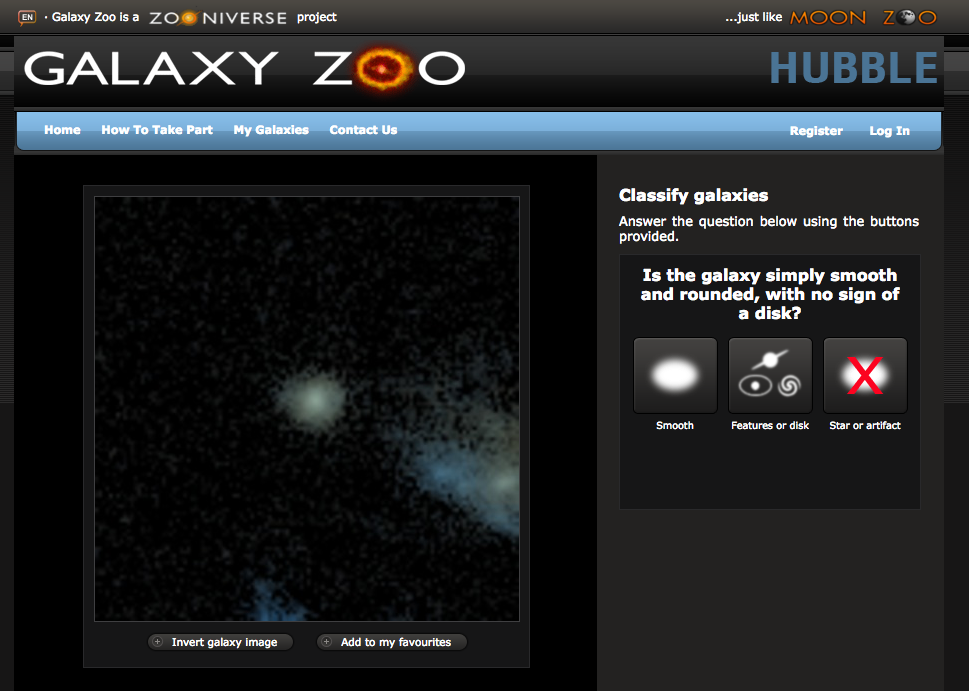
\includegraphics[width=160mm]{figures/gzh_interface.png}
\caption{Screenshot of the Galaxy Zoo: Hubble interface showing an example COSMOS image at the first step in the decision tree.\label{fig:interface}}
\end{figure*}

\section{Correcting for redshift-dependent classification bias}

The previous versions of Galaxy Zoo morphology classifications \citep{lin08,wil13} were based on observations of galaxies in the Sloan Digital Sky Survey (SDSS) which are typically at $z<0.1$. In these cases it was assumed that there was no cosmological evolution of the morphologies of galaxies and therefore any observed changes in the distribution of galaxies with different consensus morphologies was due to the effects of redshift on the image quality (\ie. the reduction in physical resolution, surface brightness dimming, etc). For both previous releases of GZ morphologies, we provided a correction for redshift-dependent bias based on matching the classification fractions at the highest redshfts with those at the lowest redshift. See \citet{bam09} and \citet{wil13} for the details. 

In the GZH samples, the redshift range is large enough that we expect to measure cosmological evolution of the types and morphologies of galaxies in the sample. As a result, the previous methods of correcting for redshift dependent bias will not work. In addition, the effects of band shifting will change the images even more across these redshift ranges. %Figure~\ref{fig:exampleFERENGI} illustrates some of the possible effects of losing features in spiral galaxies at high redshift. 

%-----------------------------------------------------------------------------------------------------------------------------------
%\begin{figure}
%\begin{center}
%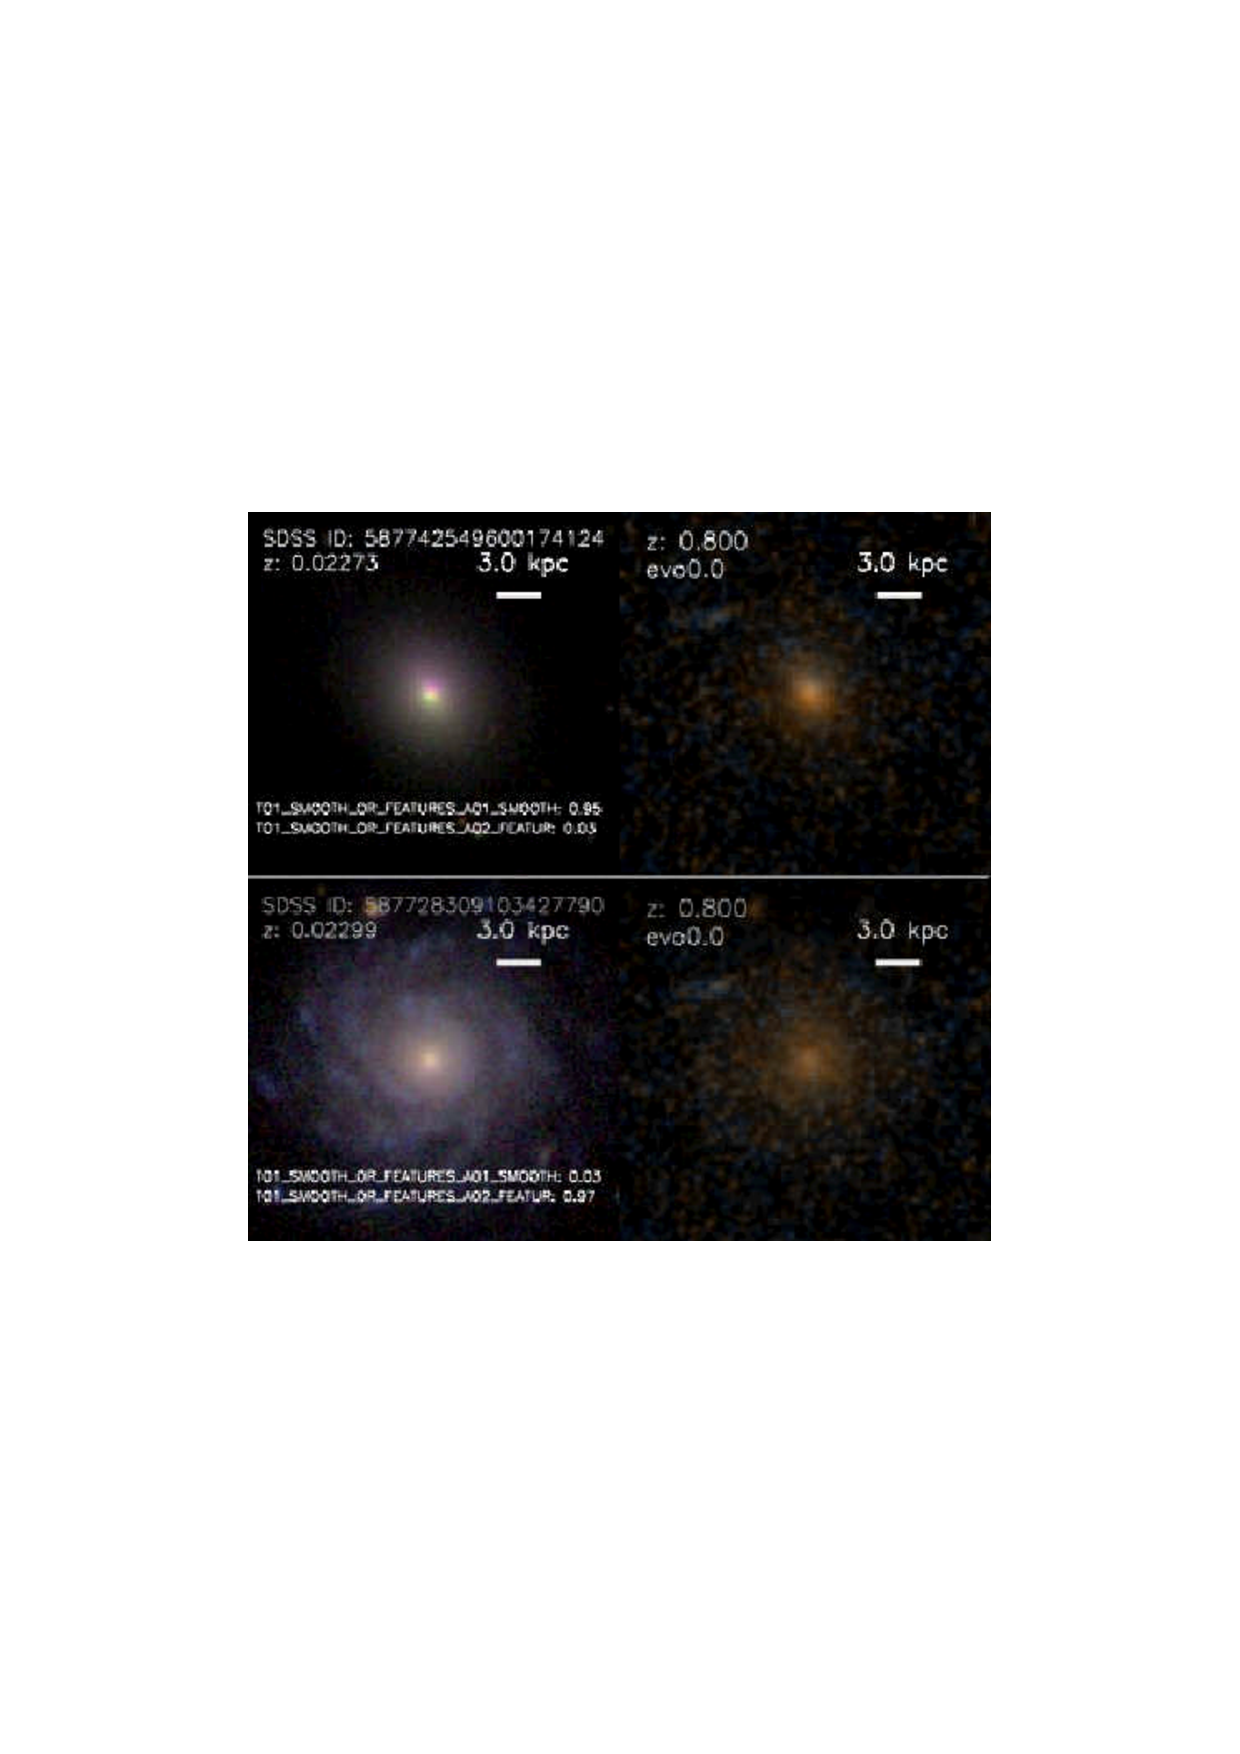
\includegraphics[width=60mm]{figures/example_ferengi2.pdf}
%\caption{Examples of an obvious spiral and obvious elliptical at $z=0$ which both look similar when redshifted to $z=0.8$. See below for the description of the method for redshifting.\label{fig:exampleFERENGI}}
%\end{center}
%\end{figure}
 %-----------------------------------------------------------------------------------------------------------------------------------

In order to test and correct for the effects of redshift, we generated a set of calibration images. These images consist of the same galaxy as it would appear over a variety of redshifts. The input images are from the SDSS \citep{yor00,str02} and are processed using the \ferengi{} code \citep{bar08a} to match the observational properties of the HST surveys out to $z=1$. These images were classified in the Galaxy Zoo interface using the same classification scheme as the original HST images.
 
\subsection{Selection of FERENGI input galaxies}

We selected 288 unique galaxies from SDSS imaging to run through the \ferengi{} code. The selection spanned a variety of galaxy morphologies (as selected by GZ2 classifications) and $r^\prime$-band surface brightnesses, and also spanned the redshift range of SDSS targets (in $N_z = 4$ bins) in order to be optimised for different target minimum redshifts in HST imaging. 

The selection criteria for the different morphological categories is summarised in Table \ref{morphologies}. The surface brightness selection ($N_\mu = 3$) was (1) low: $\mu > 21.5$~\magarc;  (2) mid: $20.5 < \mu < 21.5$~\magarc; and (3) high: $\mu < 20.5$~\magarc. For each of the four ``target redshifts'' ($z = 0.3, 0.5, 0.8$ and $1.0$), the images were redshifted in $\Delta z = 0.1$ bins up to $z=1.0$. 
 
\begin{table*}
\caption{Summary of morphological categories selected for FERENGI sample.\label{morphologies}}
\begin{tabular}{lllc}
\hline\hline
Morphology          & Label &  Selection                                                                                            & $N_{\rm objects}$ \\
                    &       &                                                                                                       & [$N_z \times N_\mu$] \\
\hline
Features            & Yes       & $p_{\rm features} > 0.8$, $p_{\rm odd} < 0.1$                                                         & 12 \\ 
                    & Int.      & $0.3 < p_{\rm smooth} < 0.6$, $p_{\rm odd} < 0.1$                                                     & 12 \\ 
                    & No        & $p_{\rm smooth} > 0.8$, $p_{\rm odd} < 0.1$                                                           & 12 \\ 
Merger              & No        & $p_{\rm features} > 0.8$, $p_{\rm odd < 0.1}$, $p_{\rm merger} < 0.1$                                 & 12 \\
                    & Int.      & $p_{\rm odd} > 0.5$, $0.1< p_{\rm merger} < 0.4$                                                      & 12 \\ 
                    & Yes       & $p_{\rm odd} > 0.5$, $p_{\rm merger} > 0.4$                                                           & 12 \\
Edge-on             & Yes       & $p_{\rm edgeon} > 0.8$, $p_{\rm features} > 0.5$                                                      & 12 \\
                    & Int.      & $0.4 < p_{\rm edgeon} < 0.8$ , $p_{\rm features} > 0.5$                                               & 12 \\
                    & No        & $p_{\rm edgeon} < 0.2$, $p_{\rm features} > 0.5$                                                      & 12 \\
Bar                 & No        & $p_{\rm bar} < 0.1$, $p_{\rm features} > 0.5$, $p_{\rm edgeon} < 0.2$                                 & 24 \\
                    & Int.      & $0.2 < p_{\rm bar} < 0.4$, $p_{\rm features} > 0.5$, $p_{\rm edgeon} < 0.2$                           & 24 \\
                    & Yes       & $p_{\rm bar} > 0.8$, $p_{\rm features} > 0.5$, $p_{\rm edgeon} < 0.2$                                 & 24 \\
Visible spiral      & No        & $p_{\rm spiral} < 0.2$, $p_{\rm features} > 0.5$, $p_{\rm edgeon} < 0.2$, $p_{\rm bar} < 0.1$         & 12 \\
                    & Int.      & $0.2 < p_{\rm spiral} < 0.8$, $p_{\rm features} > 0.5$, $p_{\rm edgeon} < 0.2$, $p_{\rm bar} < 0.1$   & 12 \\
                    & Yes       & $p_{\rm spiral} > 0.8$, $p_{\rm features} > 0.5$, $p_{\rm edgeon} < 0.2$, $p_{\rm bar} < 0.1$         & 12 \\
Oblique bulge size  & No        & $p_{\rm nobulge>0.6}$, $p_{\rm features} > 0.5$, $p_{\rm edgeon} < 0.5$, $p_{\rm bar} < 0.2$          & 12 \\
                    & Int.      & $p_{\rm justnoticeable}>0.6$, $p_{\rm features} > 0.5$, $p_{\rm edgeon} < 0.5$, $p_{\rm bar} < 0.2$   & 12 \\
                    & Yes       & $p_{\rm obvious|dominant}>0.5$, $p_{\rm features} > 0.5$, $p_{\rm edgeon} < 0.5$, $p_{\rm bar} < 0.2$ & 12 \\
Edge-on bulge shape & Round     & $p_{\rm rounded}>0.5$, $p_{\rm features} > 0.5$, $p_{\rm edgeon} > 0.5$                               & 12 \\
                    & Boxy      & $p_{\rm boxy}>0.4$, $p_{\rm features} > 0.5$, $p_{\rm edgeon} > 0.2$                                  & 12 \\
                    & No bulge  & $p_{\rm nobulge}>0.5$, $p_{\rm features} > 0.5$, $p_{\rm edgeon} > 0.5$                               & 12 \\
\hline\hline
\end{tabular}
\end{table*}

In addition to the physical parameters of the input images, the \ferengi{} output depends on assumptions of the global galaxy evolution model. This evolution is a crude mechanism that mimics the brightness increase of galaxies with increasing redshift (out to at least $z\sim1-2$). The effect on the redshifted images is simply an empirical addition to the magnitude of a galaxy of the form $M' = e\times z + M$, where $M'$ is the corrected magnitude, and $e$ is the evolutionary correction in magnitudes (i.e., $e=-1$ essentially brightens the galaxy by 1~magnitude by $z=1$). We ran \ferengi{} for values of $e$ starting from $e=0$ and decreasing to $e=-3.5$ in increments of $\Delta e = 0.5$. Figure~\ref{fig:exampleFERENGI} shows several examples of the effects of ``losing`` spiral/disc features with increasing redshift for two galaxies with $e=0$. 

The final number of \ferengi{} images produced for each galaxy is ultimately a function of galaxy's redshift, since the new images cannot be resampled at better angular resolution than the original SDSS data, as well as the number of $e$ values selected. Table~\ref{ferengivalues} summarizes the total sample of redshifted images produced for GZH. 

\begin{table}
\caption{Summary of FERENGI artificial redshifting \label{ferengivalues}}
\begin{tabular}{lccccr}
\hline\hline
$z_{\rm target}$ & $N_{z {\rm bins}}$ & $N_{\rm evolution}$ & $e_{\rm max}$ & $N_{\rm galaxies}$ & $N_{\rm images}$\\
\hline
0.3              & 8                  & 7                   & $-3.0$        & 72             & 4032 \\
0.5              & 6                  & 4                   & $-1.5$        & 72             & 1728 \\
0.8              & 3                  & 3                   & $-1.0$        & 72             &  648 \\
1.0              & 1                  & 3                   & $-1.0$        & 72             &  216 \\
\hline\hline
\end{tabular}
\end{table}

\begin{figure*}
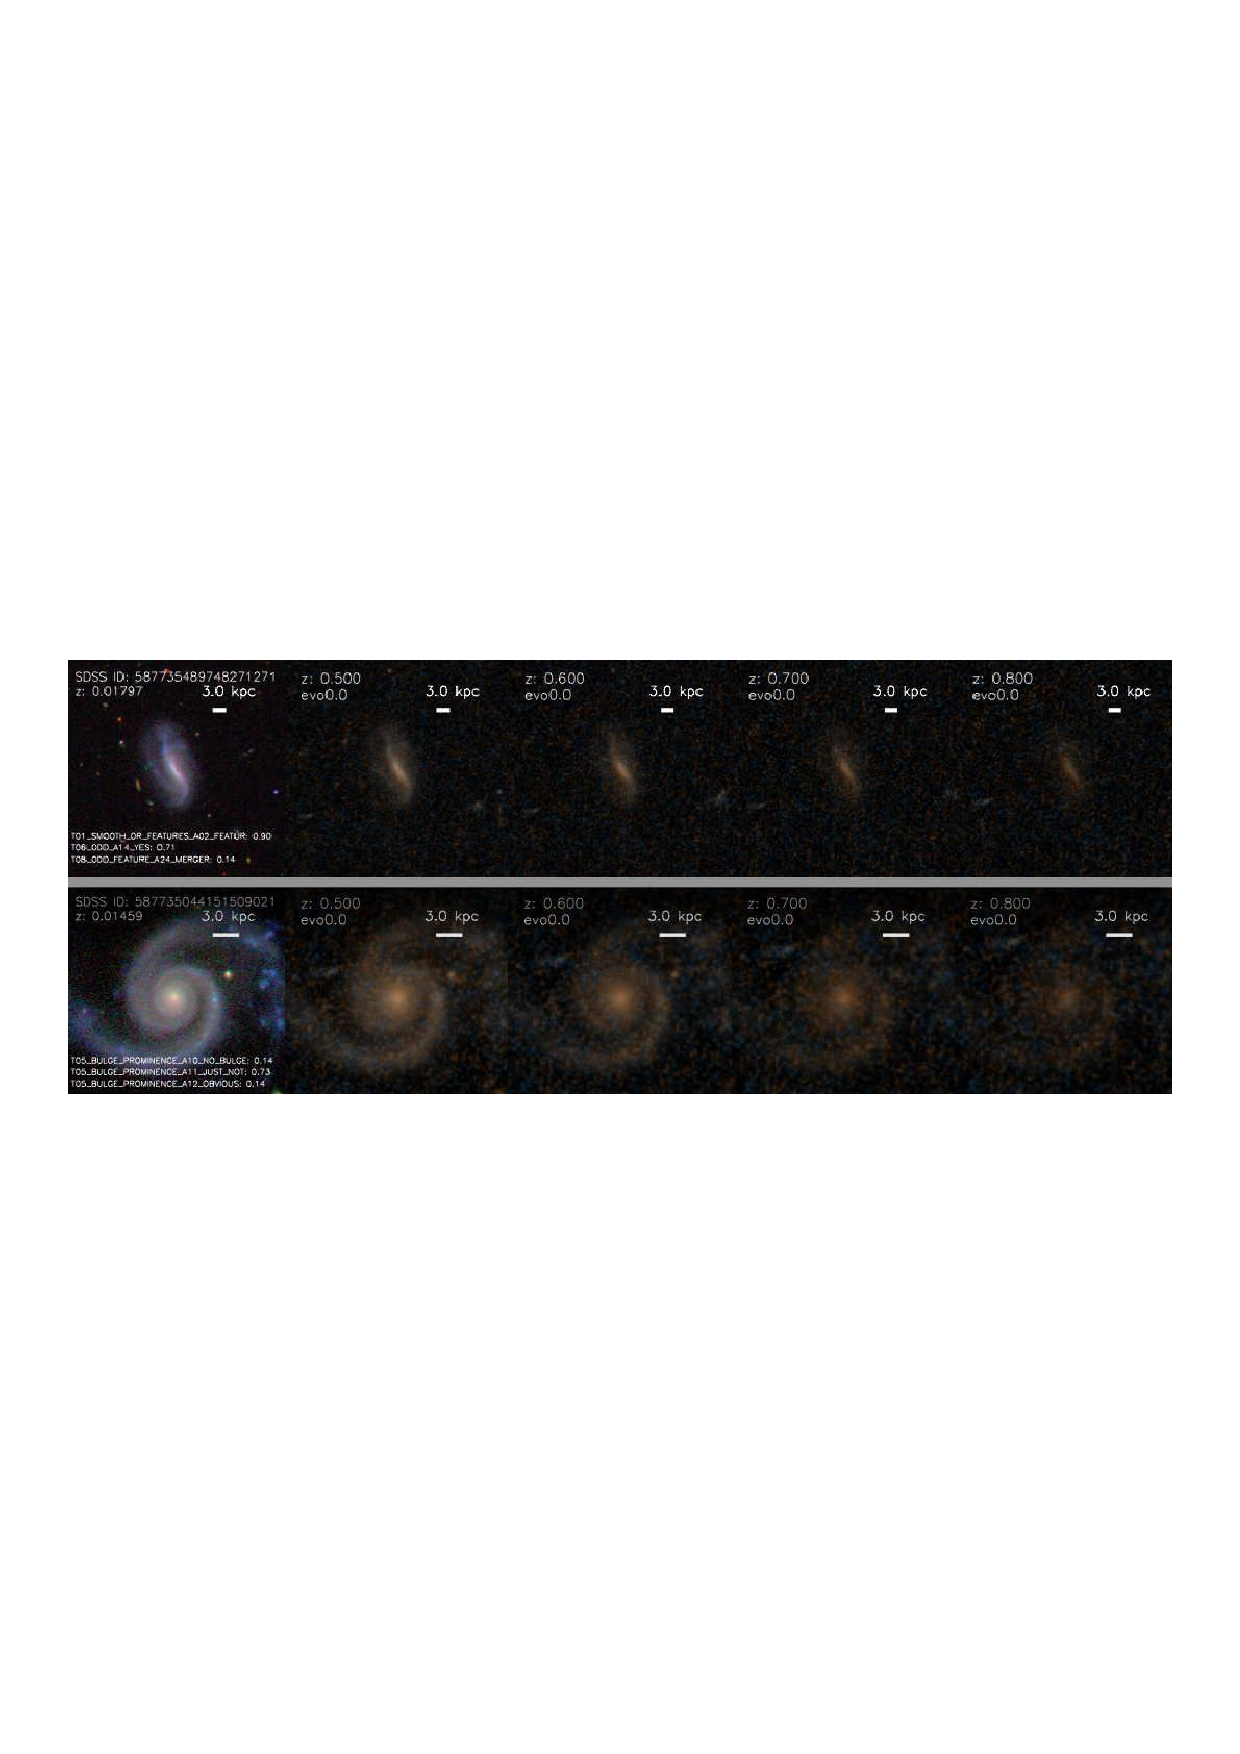
\includegraphics[width=160mm]{figures/example_ferengi.pdf}
\caption{Examples of two galaxies which have been run through the FERENGI code to produce simulated HST images. The value of $p_{\rm features}$ for each panel is (1) Top row: $p_{\rm features}=$ 0.9, 0.625, 0.35, 0.35, 0.225 and (2) Bottom row: $p_{\rm features}=$ 1.00, 0.875, 0.875, 0.625, 0.375. \label{fig:exampleFERENGI}}
\end{figure*}

\subsection{Correcting GZH morphologies for classification bias}
\label{sec:zeta}

The approach used in GZH for correcting the weighted classifications for user bias rests on the assumption that the \emph{amount} of bias is a function of the apparent size and brightness of the image as seen on screen. This is controlled by two types of parameters: \textbf{intrinsic} properties of the galaxy itself, such as its physical diameter and luminosity, and \textbf{extrinsic} properties, such as the distance (redshift) of the galaxy and its relative orientation. There are likely other parameters that affect user accuracy, such as the proximity of close companions \citep[``distraction bias''; see][]{joh15} or bias as a function of the individual user. The combination of all such parameters forms a high-dimensional space, and we have insufficient data to measure their individual effects. Instead, we use just two parameters that are intended to capture the bulk of the change in bias (based on GZ1/GZ2): a galaxy's $r^\prime$-band surface brightness ($\mu_r$; intrinsic) and redshift ($z$; extrinsic). 

The change in bias as a function of $\mu_r$ and $z$ is measured using the \ferengi{} images over all the evolutionary correction factors. We assume that the ``true'' (ie, debiased) vote fraction $f_{\mu,z}$ for a galaxy can be expressed as:

\begin{equation}
f_{\mu,z} = \left(f_{\mu,z=0.3}\right) \times e^{{\frac{z-z_0}{\zeta}}},
\label{eqn:fzeta}
\end{equation}

\noindent where $f_{\mu,z=0.3}$ is the ``calibrated'' vote fraction at the lowest redshift in the \ferengi{} bins ($z=0.3$) and $\zeta$ is a positive parameter that controls the rate at which $f$ decreases with increasing redshift. This formula fits the data relatively well (with almost no exceptions, the vote fractions for featured galaxies decrease monotonically with increasing redshift), and the exponential function bounds the observed vote fractions between $f_{\mu,z=0.3}$ and zero. Figure~\ref{fig:zeta_examples} show examples of the change in vote fraction and their fits to Equation~\ref{eqn:fzeta} for a random selection of galaxies in the \ferengi{} images. 

\begin{figure*}
\begin{center}
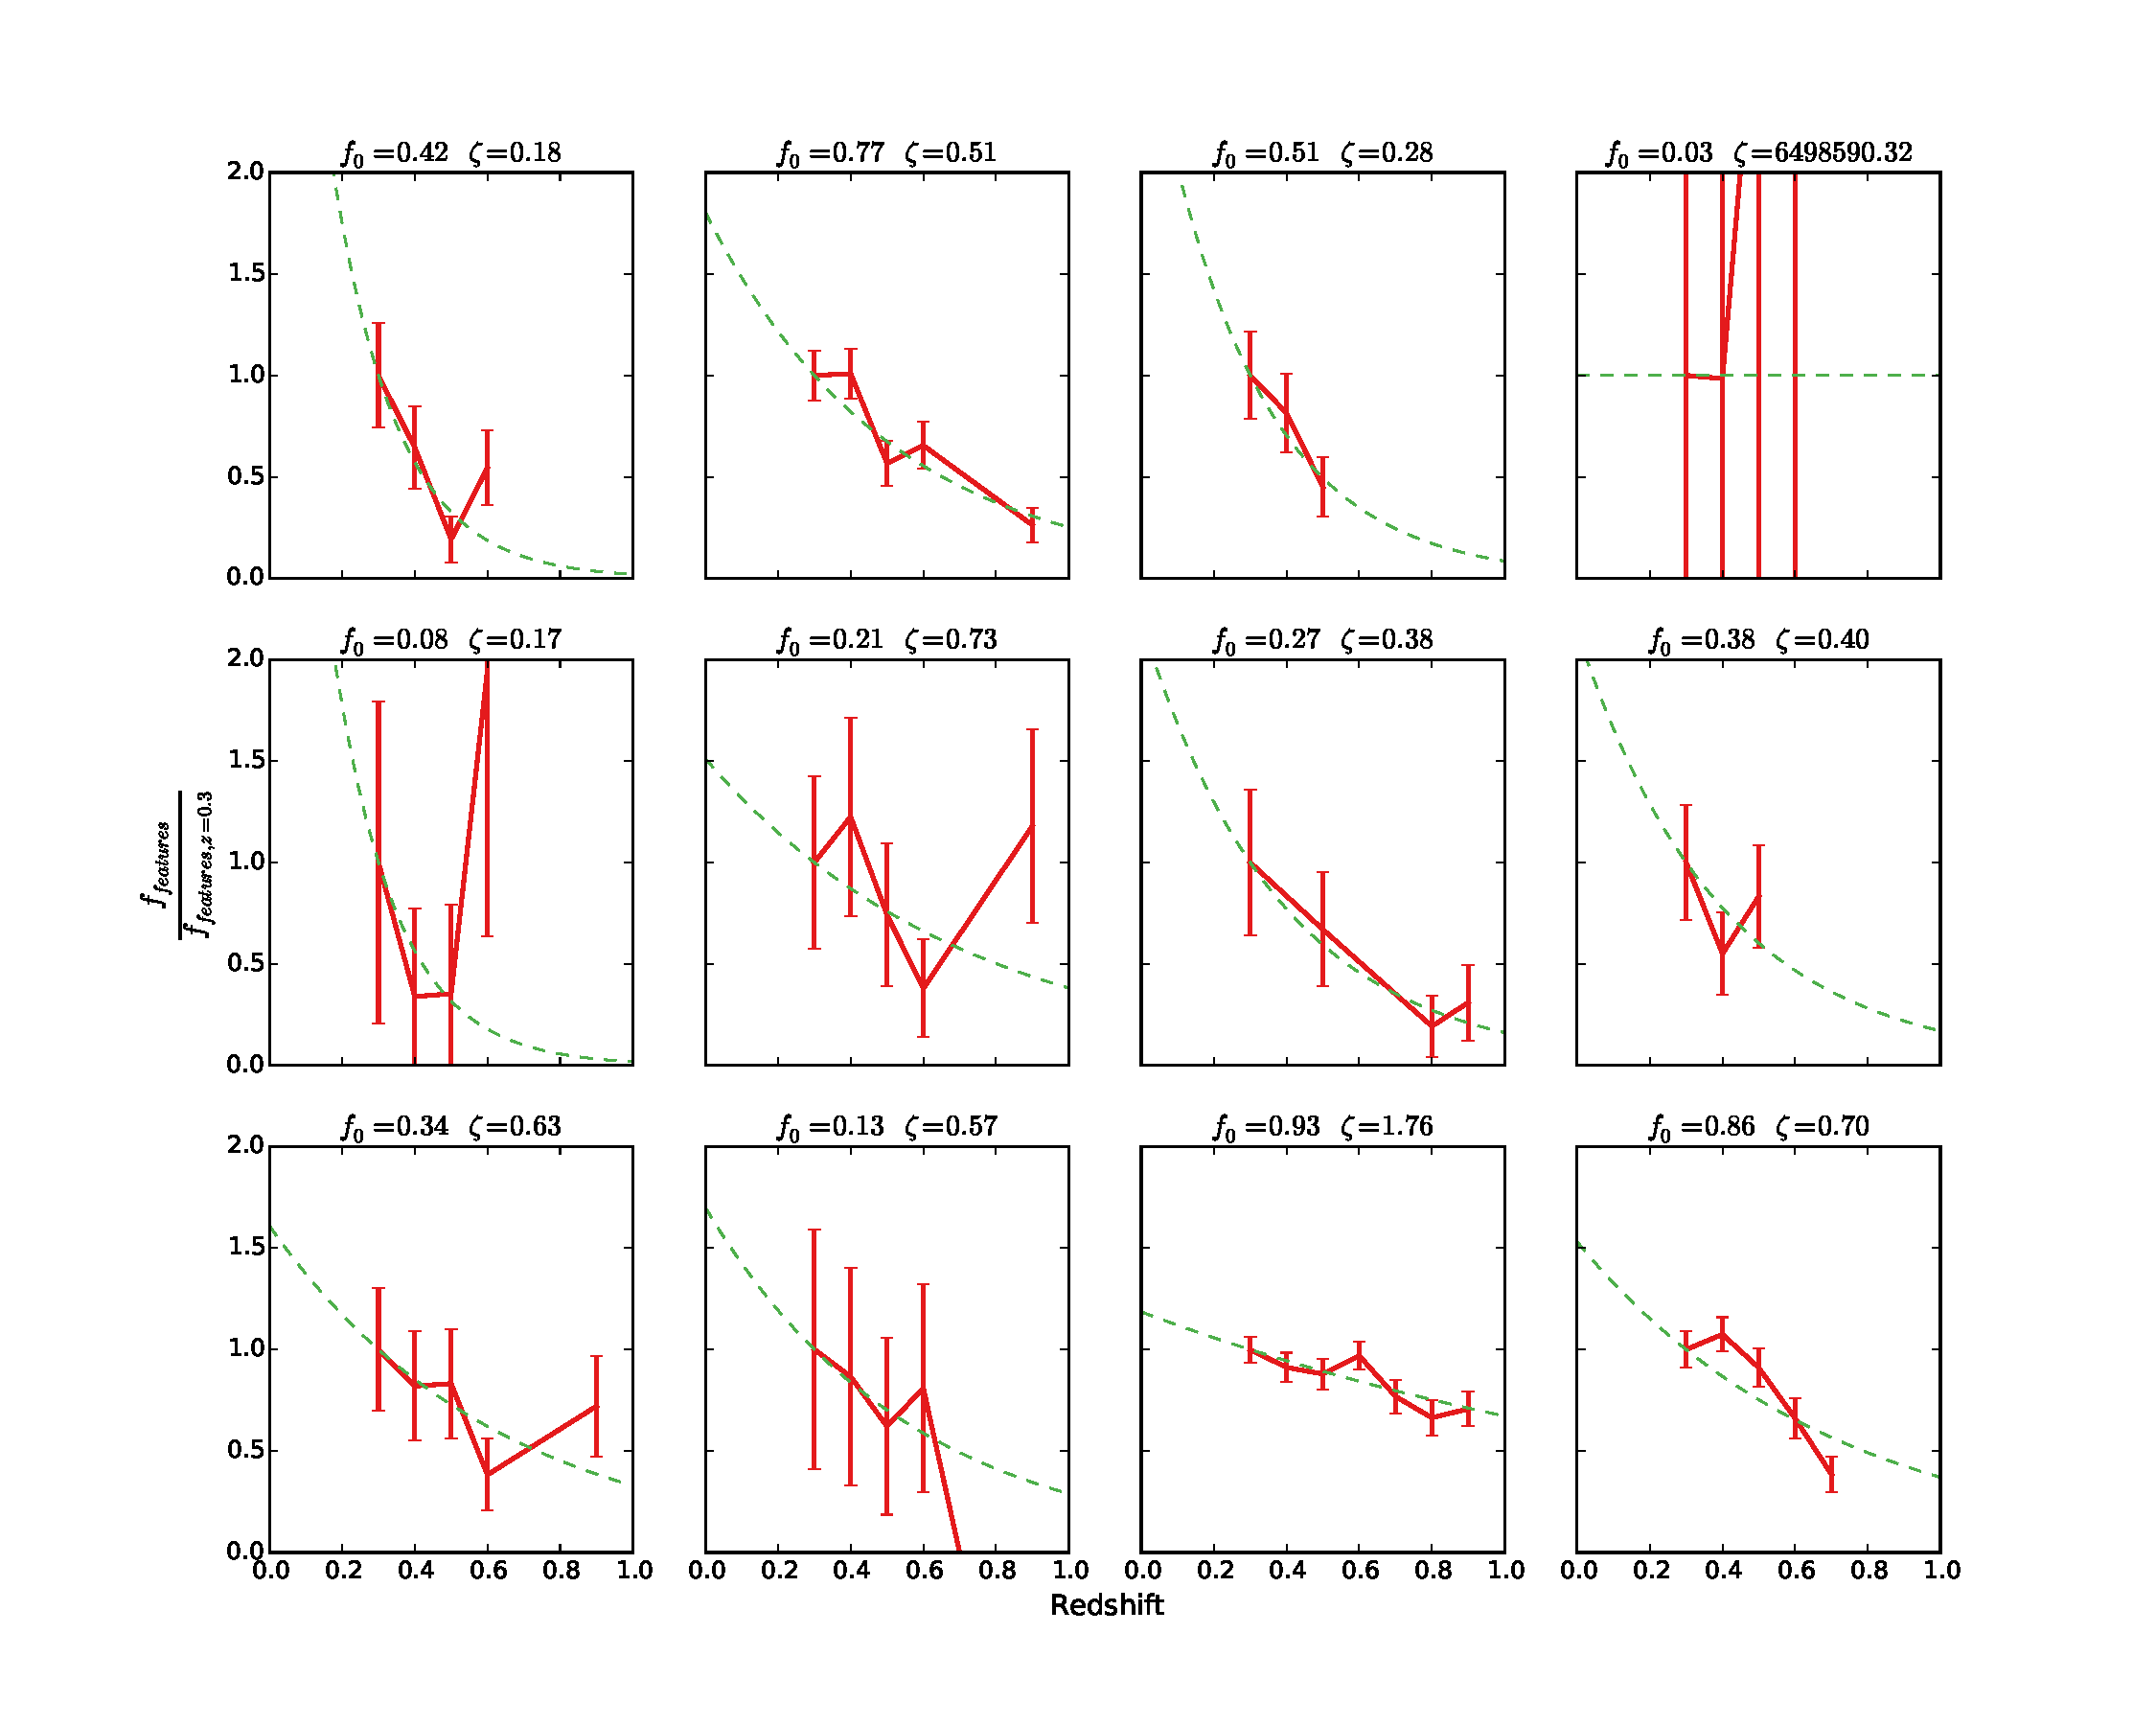
\includegraphics[width=\textwidth]{figures/zeta_examples.pdf}
\caption{Behavior of the normalized, weighted vote fractions of features visible in a galaxy ($f_\textrm{features}$) as a function of redshift in the artifical \ferengi{} images. Galaxies are a random selection of images with $e=0$ and at least three detectable images in redshift bins of $z\ge0.3$. The measured vote fractions (red points) are fit with an exponential function (Equation~\ref{eqn:fzeta}); the best-fit parameters are given above each plot. Error bars are Poissonian, assuming a median of 40~votes per galaxy.}
\label{fig:zeta_examples}
\end{center}
\end{figure*}

We use the values of $\zeta$ for \emph{all} sets of artifically redshifted galaxies to fit the overall distribution as a function of surface brightness, since we expect the correction being applied to vary as a function of the intrinsic galaxy properties. We restrict the galaxies that can be used to measure the calibration to those with data at the pivot redshift of $z=0.3$, non-zero $f_\textrm{features}$ at $z=0.3$, and with a reasonable fit to the exponential model ($\Delta \chi^2 > 3.0$). 

Figure~\ref{fig:zeta_mu} shows the results of fitting the \ferengi{} images with Equation~\ref{eqn:fzeta}; the correction is a weak function of galaxy surface brightness. Higher-surface brightness galaxies have stronger average corrections, likely because these galaxies are more likely to have larger $f_\textrm{features}$ values at high redshifts. Low surface brightness galaxies are more likely to begin low and remain low; the bounded nature of the dropoff (and Poissonian-like variance among the individual voters) means that the average magnitude of $\zeta$ will be less. 

\begin{figure}
\begin{center}
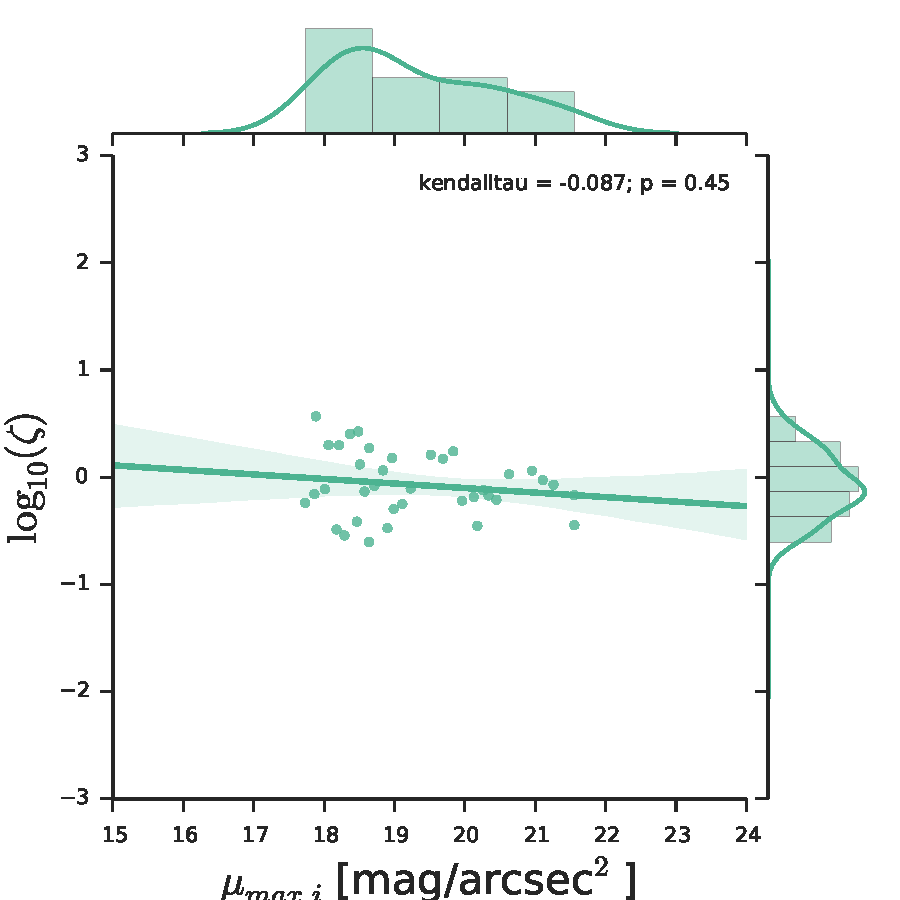
\includegraphics[width=0.50\textwidth]{figures/zeta_mu.pdf}
\caption{All fits for the vote fraction dropoff parameter $\zeta$ for $f_\textrm{features}$ in the \ferengi{} galaxies as a function of surface brightness. This includes only the 51~galaxies with a reasonably bounded range on the dropoff ($-10<\log(\zeta)<10$) and sufficient points to fit the function.}
\label{fig:zeta_mu}
\end{center}
\end{figure}

We fit the data in Figure~\ref{fig:zeta_mu} with a linear function such that:

\begin{equation}
\log_{10}(\hat\zeta) = \zeta_0 + \zeta_1 \times \mu,
\label{eqn:zetafit}
\end{equation}

\noindent where $\hat\zeta$ is the correction factor applied to each galaxy as a function of surface brightness. The best-fit parameters to the linear fit (from least-squares optimization) are $\zeta_0=0.1$, $\zeta_1=1.4$. To make the final debiased correction, we modify the simple exponential form of Equation~\ref{eqn:fzeta} to bound the debiased vote fractions between $f$ and 1:

\begin{equation}
f_\textrm{features,debiased} = 1 - (1 - f)e^{\frac{z-z_0}{\hat\zeta}}.
\label{eqn:fzeta_mod}
\end{equation}

\subsection{Results of $\zeta$ approach}

\begin{figure*}
\begin{center}
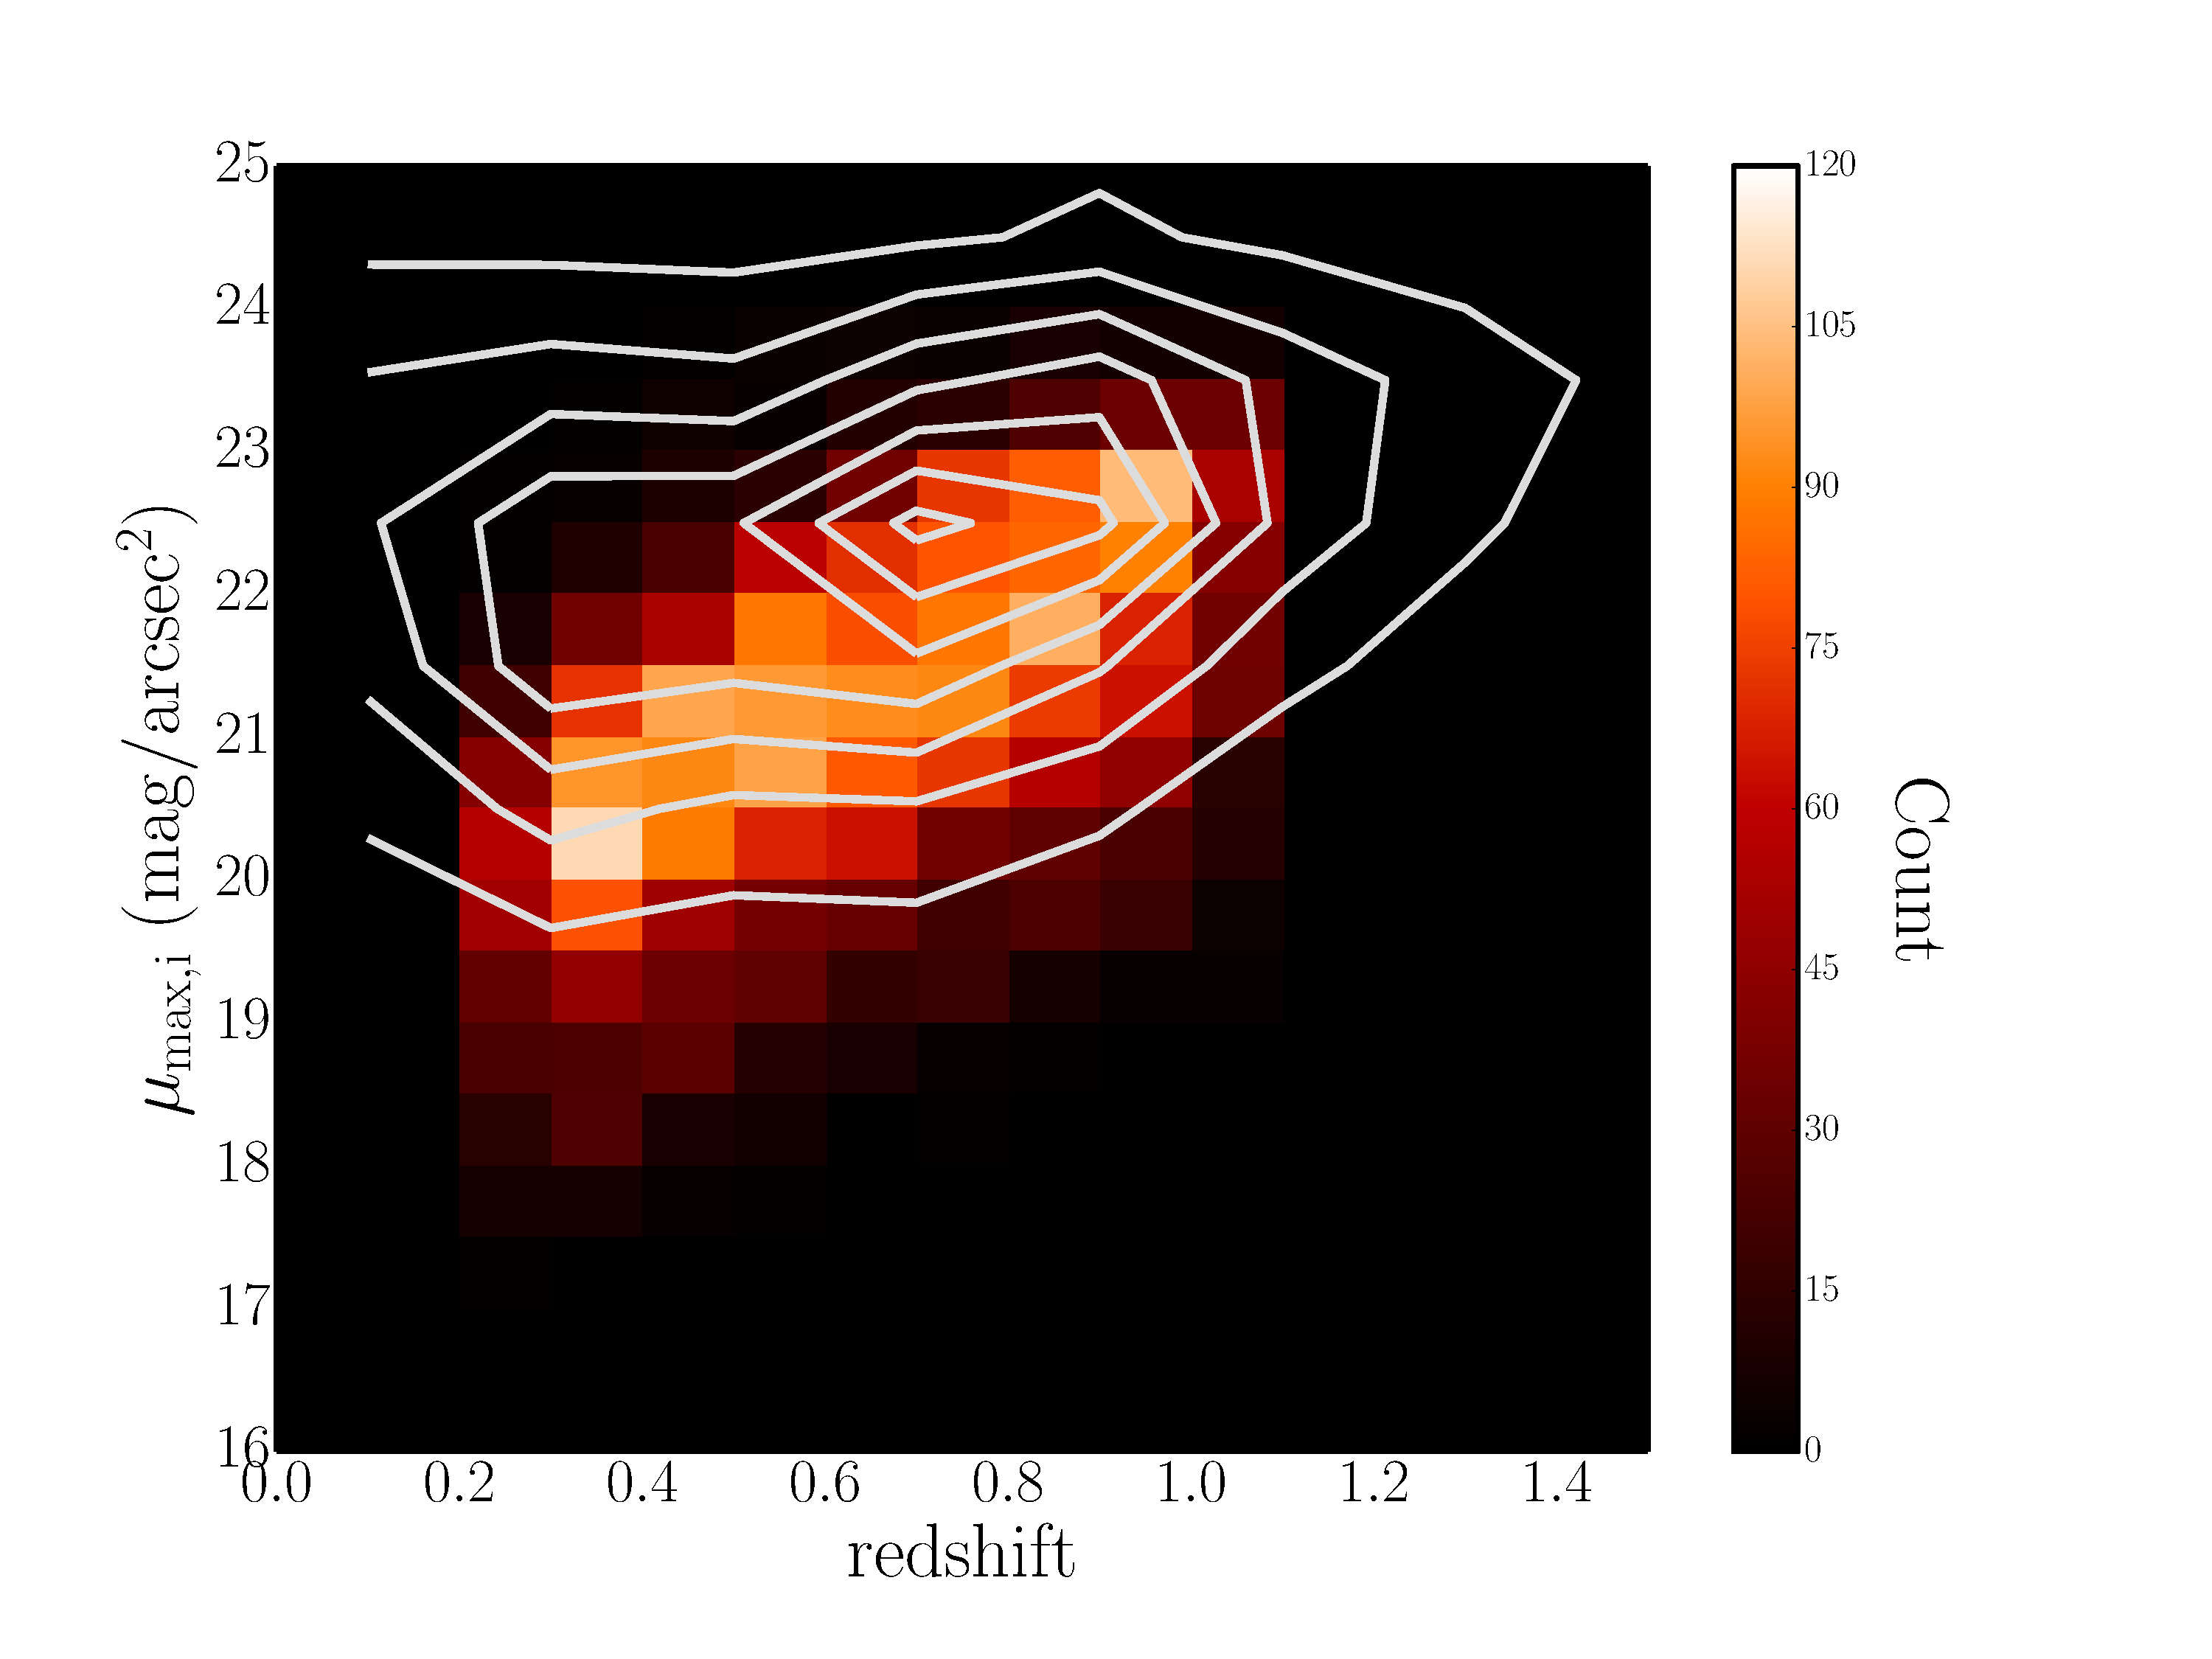
\includegraphics[width=\textwidth]{figures/eye_of_sauron.pdf}
\caption{Surface brightness vs. redshift of 118,083 galaxies in the ACS sample. The white grid denotes the surface brightness and redshift range of the \ferengi{} images, subdivided in bins corresponding to fixed ranges used for analysis in Figure~\ref{fig:p_vs_p}.}

\label{fig:features_corrections}
\end{center}
\end{figure*}

\begin{figure*}
\begin{center}
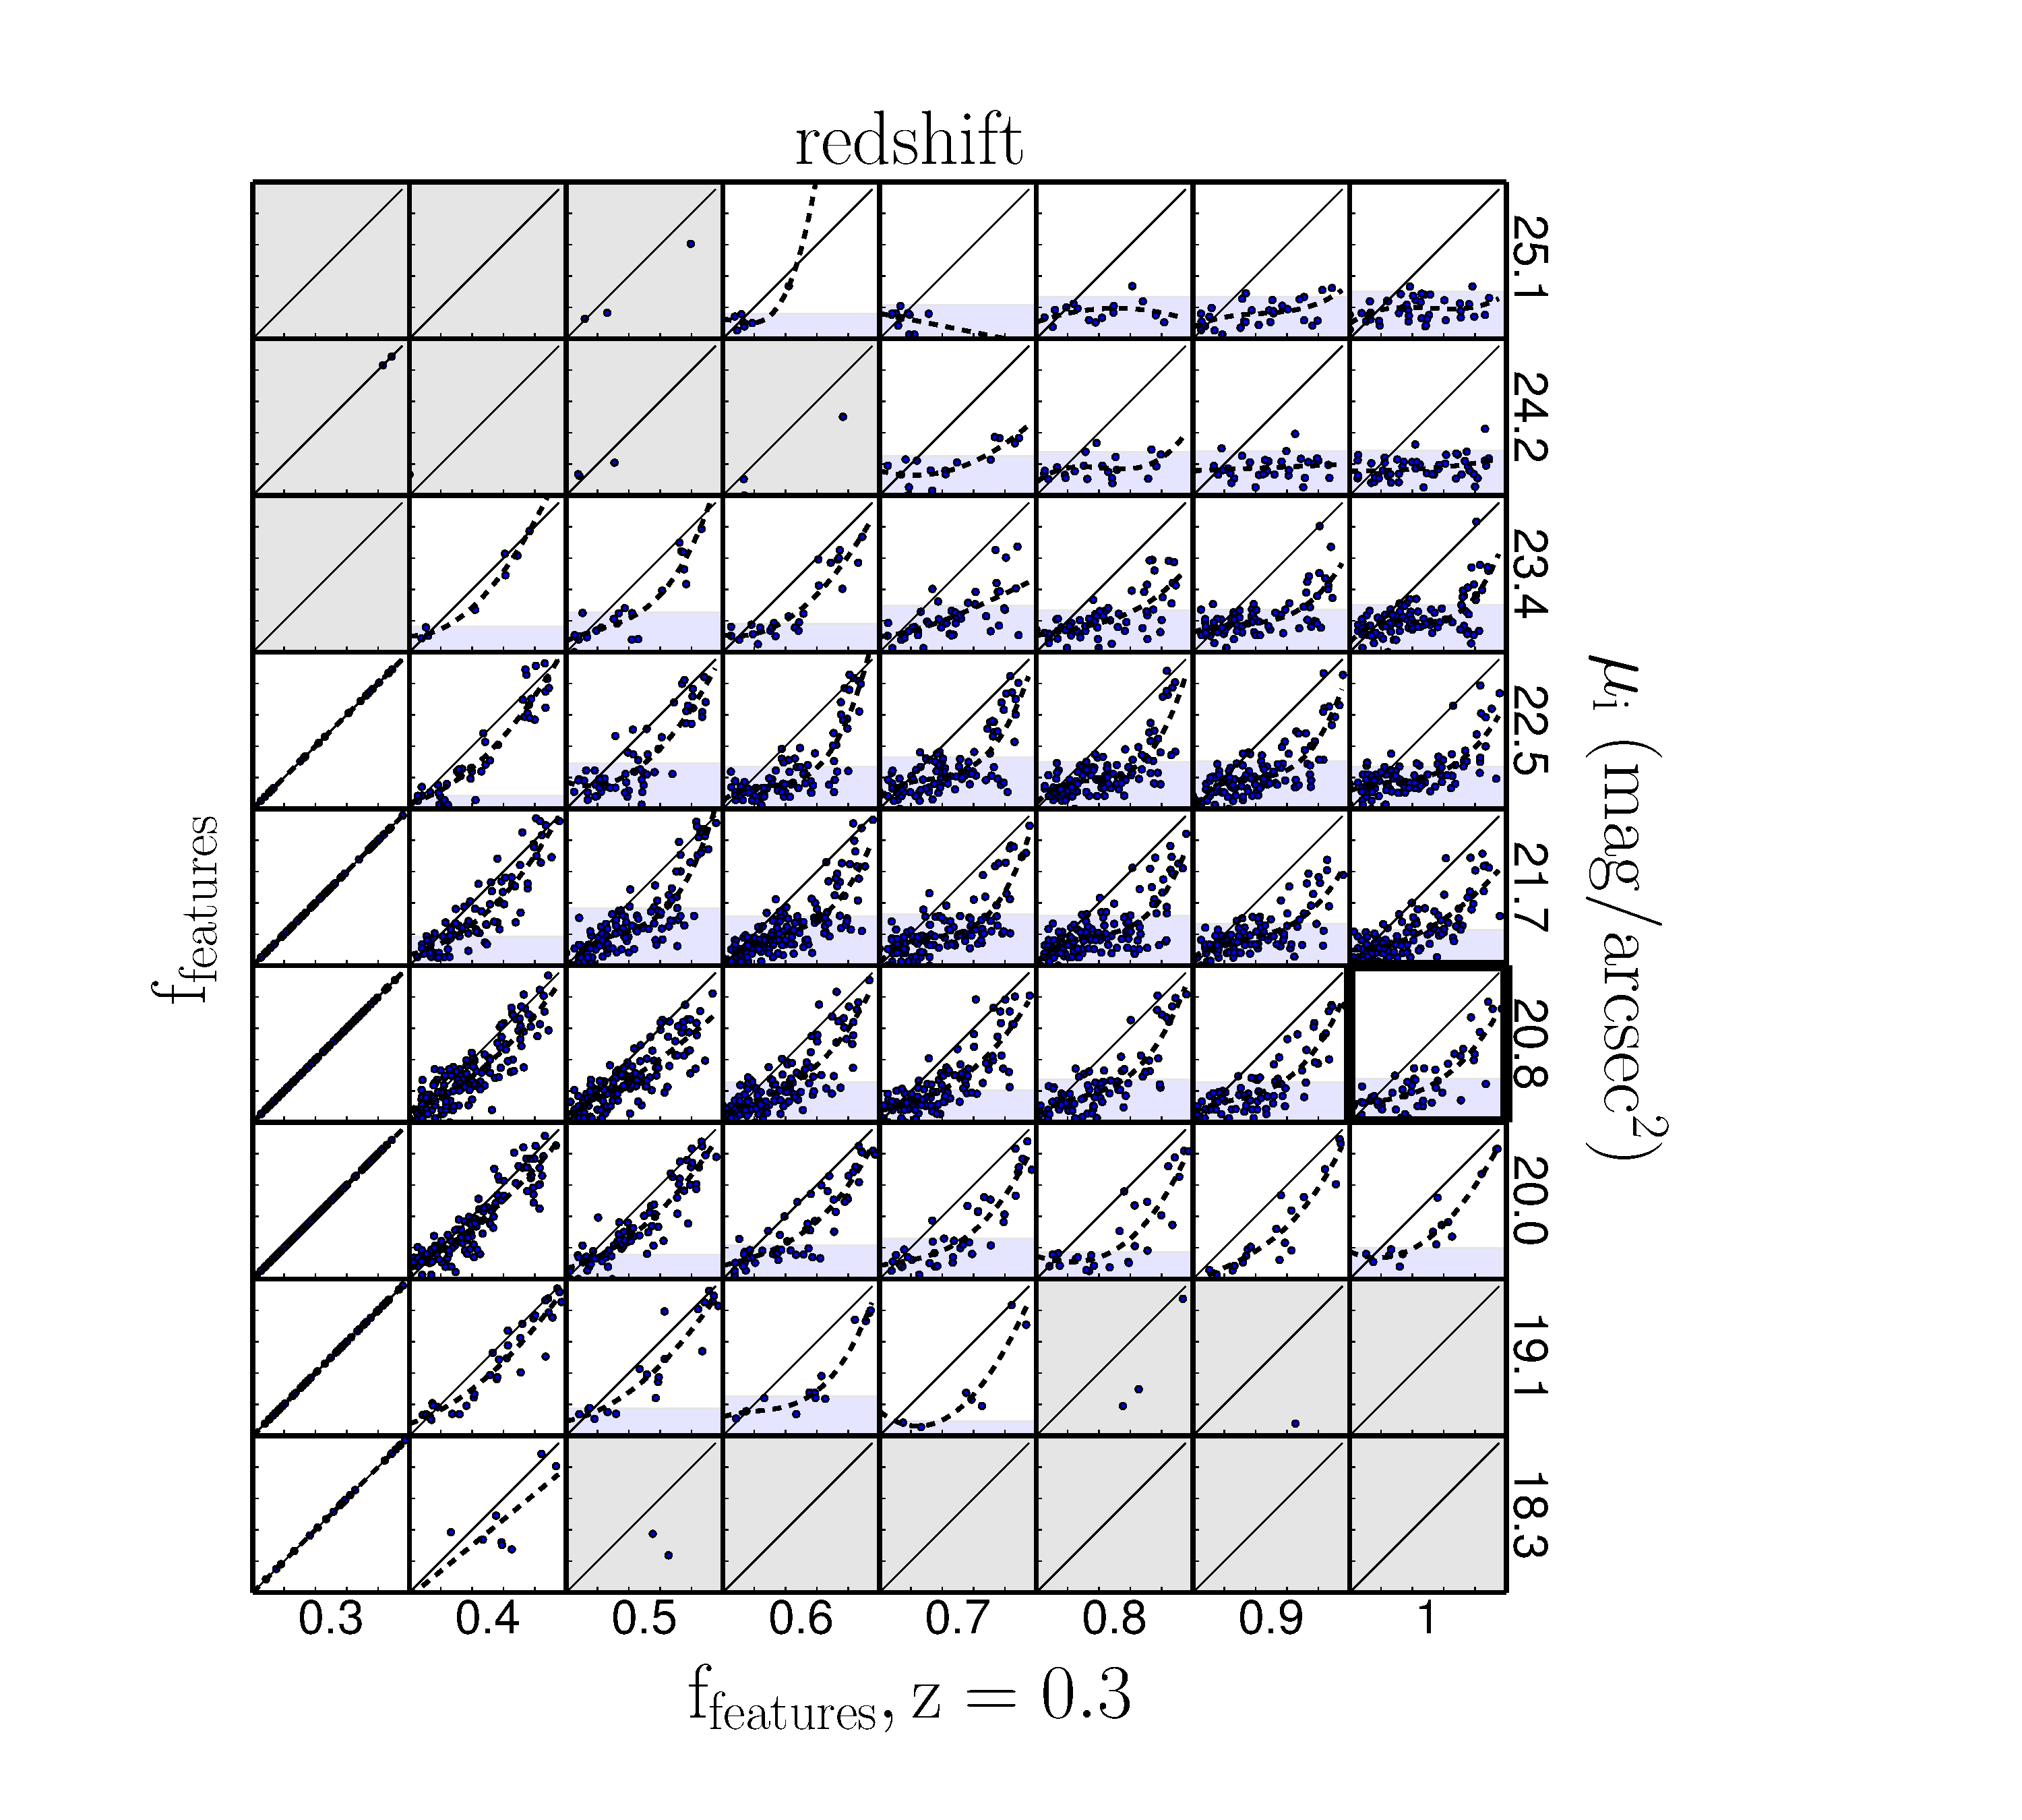
\includegraphics[width=\textwidth]{figures/p_vs_p_SB_redshift.pdf}
\caption{Effects of redshift bias in 3,959 images in the \ferengi{} sample. Each point in a given redshift and surface brightness bin represents a unique galaxy. On the y-axis in each bin is the $p_{features}$ value of the image of that galaxy redshifted to the value corresponding to that redshift bin. On the x-axis is the $p_{features}$ value of the image of the same galaxy redshifted to $z=0.3$. Regions in which there is a nearly one-to-one relationship between $p_{features}$ at high redshift and $z=0.3$ are white; those in which there is not are green, and those with not enough data ($N<5$) are purple. }
\label{fig:p_vs_p}
\end{center}
\end{figure*}

In Figure~\ref{fig:p_vs_p} we examine the change in $p_{\rm features}$ for the \ferengi{} galaxies relative to their lowest simulated redshift. In this analysis, only galaxies whose lowest simulated redshift image was ($\rm z_{sim}=0.3$) were used (see Table \ref{ferengivalues}), and only those which had detectable surface brightness measurements in \sextractor{}; this includes 3,959 of the total 6,466 images. For each simulated redshift value $z$, and at a fixed surface brightness $\mu$, we plot $p_{\rm features,z}$, the value measured at that simulated redshift, vs $p_{\rm features,z=0.3}$, the value measured for the same galaxy imaged at $z=0.3$. 
 
Our objective is to use these data to predict, for a galaxy with a measured $p_{\rm features,z}$ value, what its $p_{\rm features}$ value \emph{would have been} if it had been viewed at $z=0.3$. This predicted value is defined as the debiased vote fraction $p_{\rm features,debiased}$, and is calculated by applying a correction to the measured value of $p_{\rm features}$, determined by the $\zeta$ function described in the previous section. A reliable predicted value can be obtained so long as the relationship between $p_{\rm features,z}$ and $p_{\rm features,z=0.3}$ is single-valued; that is, for a given $p_{\rm features,z}$, there is exactly one corresponding value of $p_{\rm features}$ at $z=0.3$. 

Figure~\ref{fig:p_vs_p} shows that the relationship between $p_{\rm features,z}$ and $p_{\rm features,z=0.3}$ is \emph{not} always single valued; hence, it is not appropriate to correct galaxies that lie in certain regions of surface brightness/redshift/$p_{\rm features}$ space. These regions tend to have low $p_{\rm features}$ values at high redshift, but a wide range of values at $z=0.3$. These regions contain two morphological types of galaxies: First are genuine ellipticals, which have low values of $p_{\rm features}$ at both high and low redshift. Second are disks whose features become washed out at high redshift; hence their $p_{\rm features}$ value at $z=0.3$ may be quite high, while the value observed at high redshift is very low. This effect is strongest at high $z$ and low $\mu$, where features become nearly impossible to discern in the images.

Our criteria for determining whether a region of this space is single-valued, and therefore correctable, is as follows: For each surface brightness and redshift bin, we examine the distribution of $p_{\rm features,z=0.3}$ in four bins of $p_{\rm features,z}$. These sub-bins are marked by the horizontal lines within each larger, surface brightness/redshift bin in Figure~\ref{fig:p_vs_p}. First, we compute the interquartile range (IQR) of the distribution of $p_{\rm features,z=0.3}$ in each sub-bin, which are indicated by the orange bars. For the region to be considered correctable, we require that the IQR of the distribution within these sub-bins is less than the sub-bin height. Regions which fit these criteria are uncouloured in the plot. If the IQR is greater than the bin height, the region is considered uncorrectable; these are marked in green. Any region with fewer than 5 points is considered to have ``not enough information (NEI)'', and are shown in purple. 

Using this approach, 52\% of the \ferengi{} images were found to have single-valued relationships between their $p_{\rm features}$ values at high and low redshift (see Table \ref{ferengi_corrections} for a summary.) Only these images were used in determining the $\zeta$ function (Section \ref{sec:zeta}).  


\begin{table}
\caption{Distribution of \ferengi{} images analysed in Figure~\ref{fig:p_vs_p}. Correctable images had a single-valued relationship between their measured $p_{\rm features}$ values at high and low redshifts (white regions in Figure~\ref{fig:p_vs_p}). Uncorrectable images had a non single-valued relationship (green regions). NEI images had undetermined relationships due to a lack of data ($N<5$) in their corresponding sub-bins (purple regions).   \label{ferengi_corrections}}
\begin{tabular}{lcc}
\hline \hline
				                   & N       & \% \\
\hline 
Correctable                        & 2,057   & 52\% \\
Uncorrectable                      & 1,732   & 44\% \\
NEI                                & 170     &  4\%\\
Total                              & 3,959   & 100\% \\
\hline \hline
\end{tabular}
\end{table}


Stuff to do in this section: 

\begin{itemize}
\item talk about where the Hubble sample falls in this space, reference table \ref{hubble_debiasable} 
\item justify $N>5$ and spread $< 0.2$ (or find a better way to choose criteria)
\item check out corrections for correctable and NEI, show some sample images of corrected galaxies
\item show some data for $\pbar$, determine or justify why we won't debiase them  
\end{itemize}

 
\begin{table*}
\caption{Breakdown of what we can correct out of the GZH data, by sample. \label{hubble_debiasable}}
\begin{tabular}{lrrrrrrr}
\hline\hline
                                   & AEGIS   & COSMOS & GEMS & GOODS-N & GOODS-S & SDSS    & Total \\
\hline
Correctable                        & 2,325   & 20,669 & 2,748 & 1,074  & 1,022   & 0       & 27,838\\
Uncorrectable                      & 1,403   & 19,626 & 1,832 & 271    & 980     & 0       & 24,112\\
No Correction Needed ($z \le 0.3$) & 967     & 11,693 & 1,190 & 280    & 247     & 37,545  & 51,922\\ 
NEI                                & 2,465   & 33,727 & 1,886 & 691    & 2,023   & 0       & 40,792\\
No Redshift Information            & 1,347   & 7,093  & 1,648 & 235    & 641     & 14,316  & 25,280\\
Total                              & 8,507   & 92,808 & 9,304 & 2,551  & 4,913   & 51,861  & 169,944\\
\hline\hline
\end{tabular}
\end{table*}

\begin{figure*}
\begin{center}
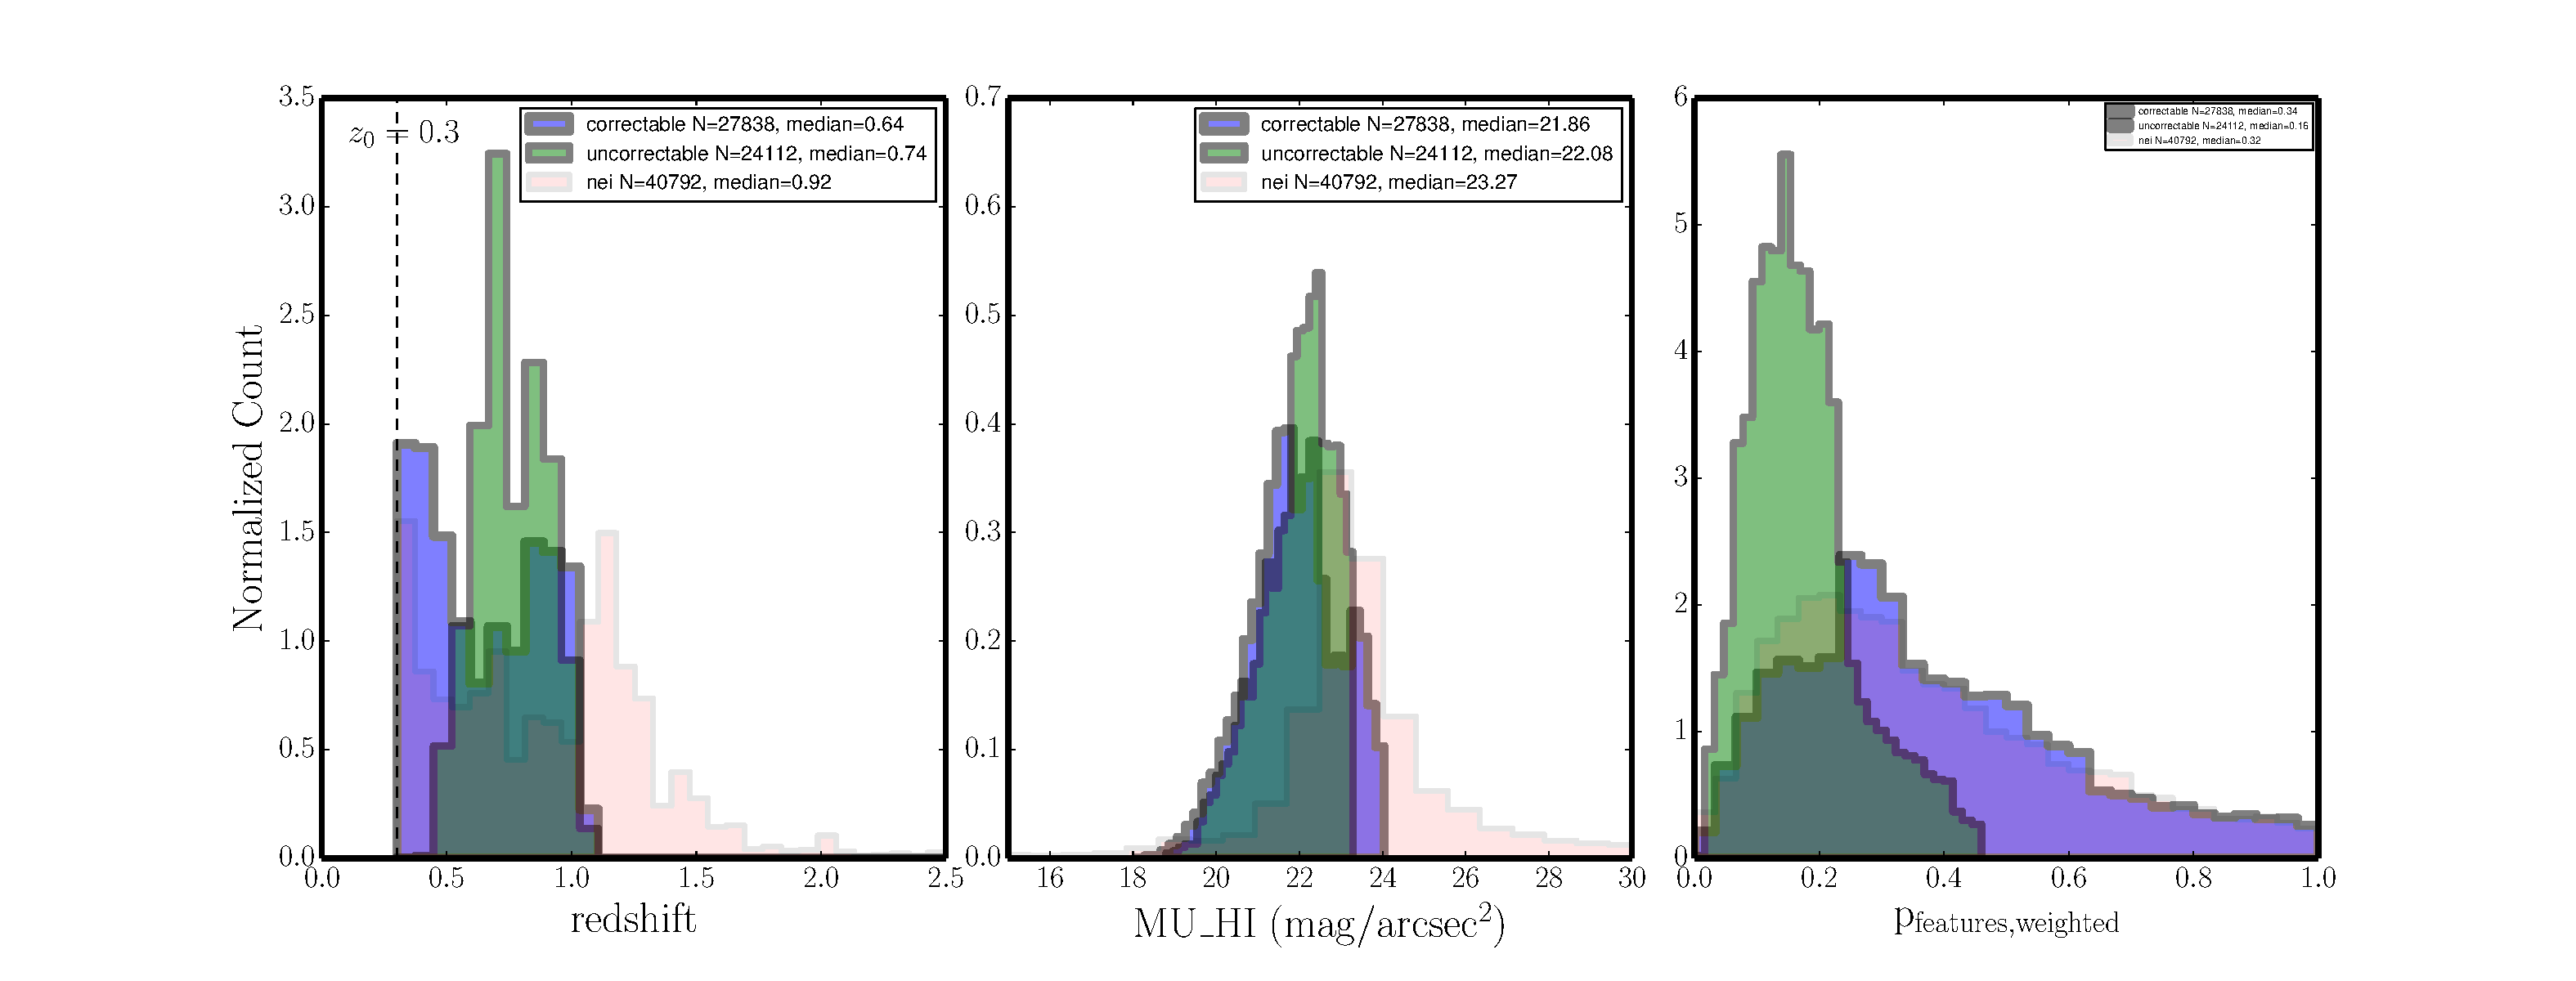
\includegraphics[width=\textwidth]{figures/hubble_z_mu_p_distributions.pdf}
\caption{Distributions of redshift, surface brightness, and $p_{features}$ for correctable (purple), uncorrectable (green), and NEI (pink) galaxies in the full GZH sample. The uncorrectable galaxies tend towards higher redshift, slightly lower in surface brightness, and lower values of $p_{features}$ than the correctable galaxies. The long tail of NEI galaxies in redshift and surface brightness demonstrates the limits of the \ferengi{} sample, for which there is no data at $z>1$ or $\mu>24$.}
\label{fig:z_mu_p}
\end{center}
\end{figure*}

\begin{figure*}
\begin{center}
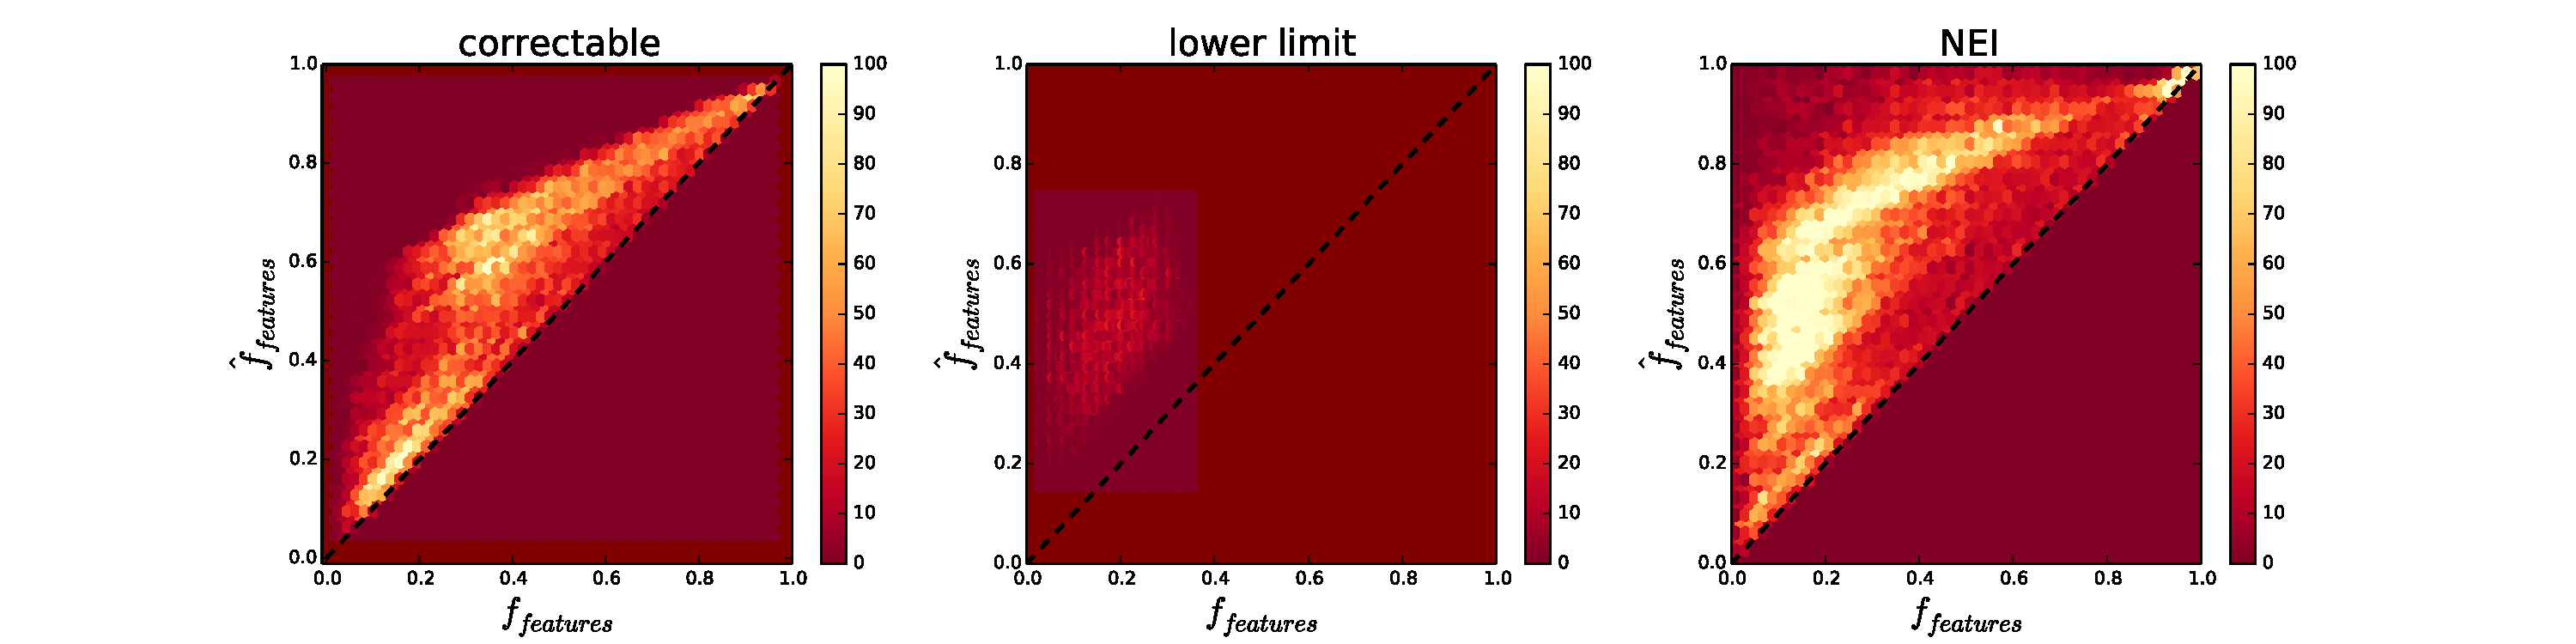
\includegraphics[width=\textwidth]{figures/debiased_corrections.pdf}
\caption{Debiased $p_{features}$ corrected to $z=0.3$ vs weighted $p_{features}$ for the correctable (left), uncorrectable (middle), and NEI (right) galaxies in the GZH sample.}

\label{fig:features_corrections}
\end{center}
\end{figure*}


%\subsection{Results of FERENGI analysis}
%
%{\bf Old text from Taiwan workshop}
%
%We show here the preliminary results of GZH classifications of images of galaxies placed at artificial redshifts. Figure~\ref{fig:ferengi_results_fake} shows the range of change of vote fractions for the change of $p_{\rm features}$ with redshift, for galaxies with different vote fraction levels, three ranges of surface-brightness levels and 7~evolutionary corrections (this last bit is indicated by the colour). 
%
%%-----------------------------------------------------------------------------------------------------------------------------------
%\begin{figure}
%\begin{center}
%
%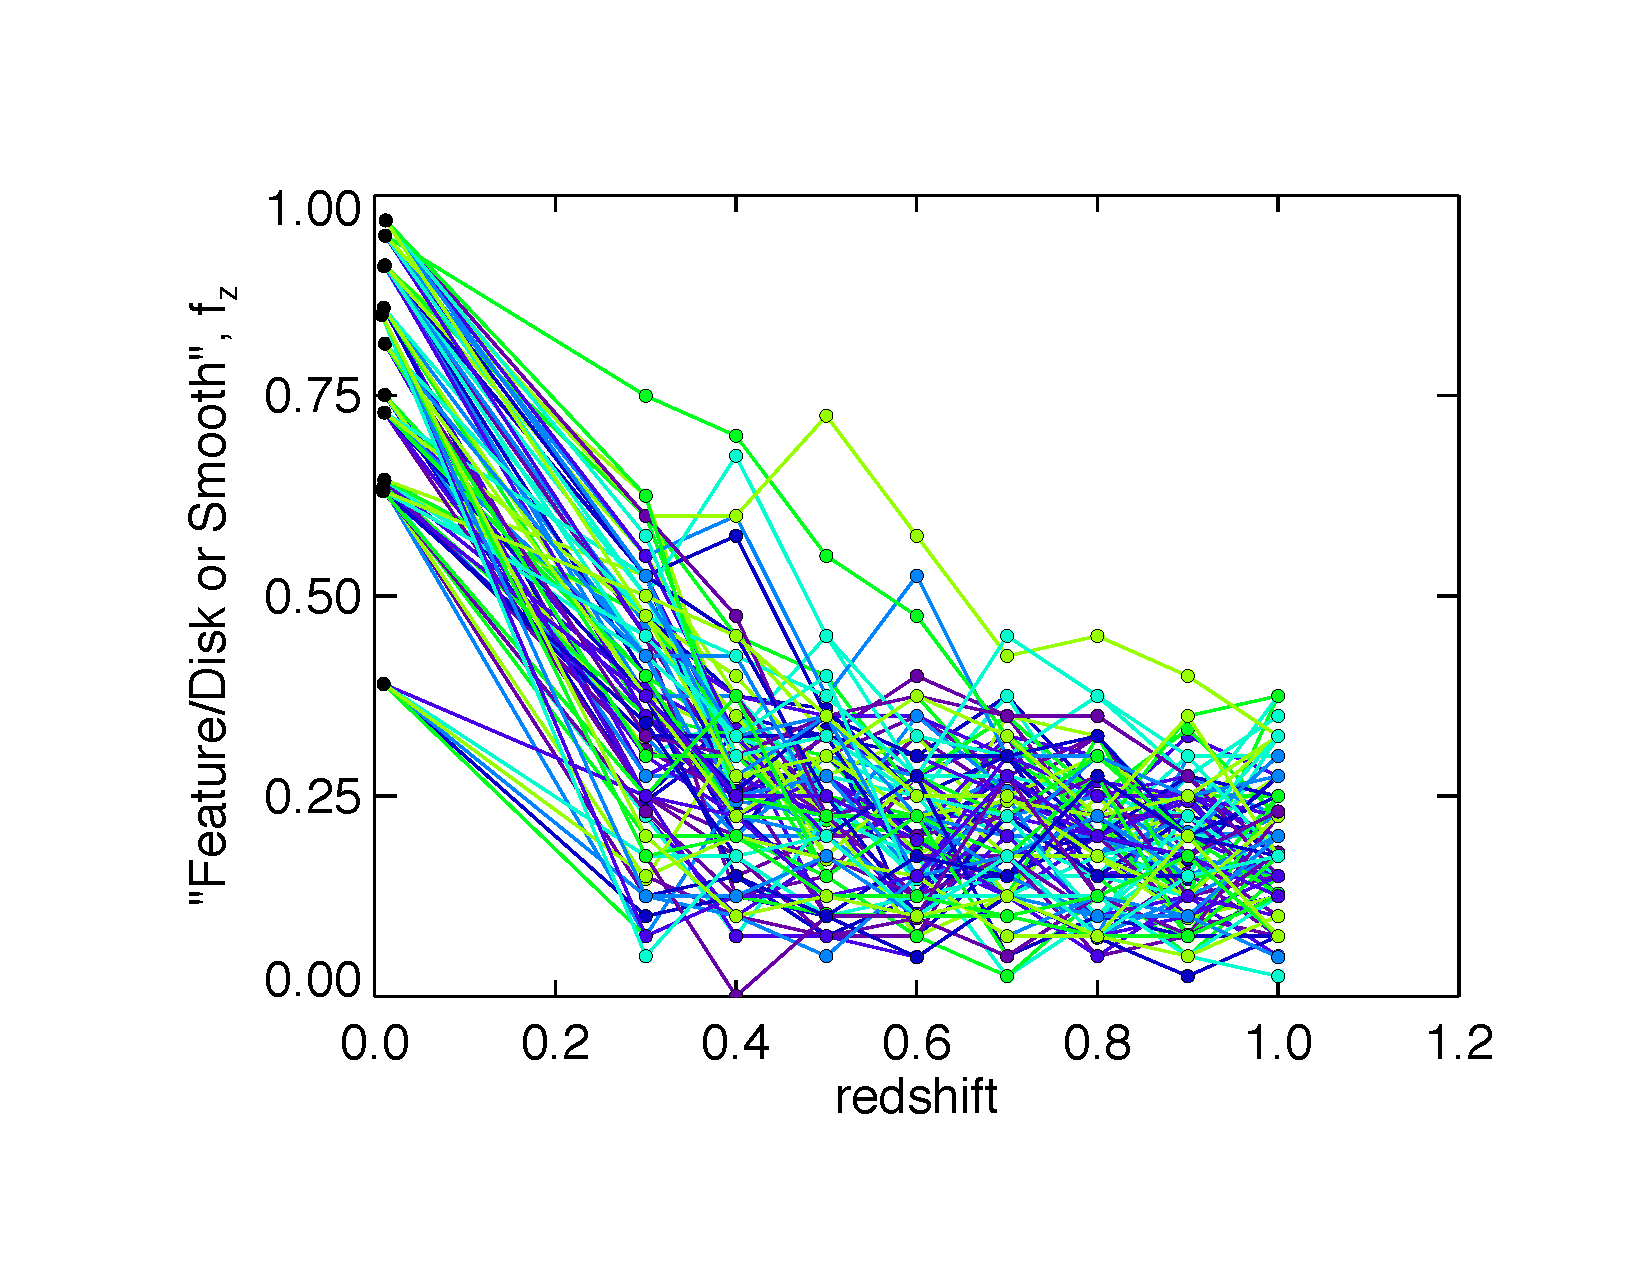
\includegraphics[width=0.45\textwidth]{figures/somewhat_fake_results.pdf}
%
%\caption{Preliminary results of the \ferengi{} redshifting exercise. WARNING NO USER WEIGHTING.... For a range of vote fraction levels with three surface-brightness levels and 7 evolutionary corrections each (the colours indicate evolutionary correction value with green being $e=0$, we show the range of evolution of the vote fractions for featured vs. smooth with redshift.}
%
%\label{fig:ferengi_results_fake}
%
%\end{center}
%\end{figure}
%%-----------------------------------------------------------------------------------------------------------------------------------


\subsubsection{TODO LIST}
We need to do: 
\begin{itemize}
\item Calculate the magnitudes, surface brightnesses and sizes of the galaxies in the FERENGI images....
\item Plot of magnitude distribution of galaxies in each of the four GZH subsamples with the magnitudes of our fake galaxies over plotted. 
\item Instructions of how to link the $z=0$ $p_X$ values for galaxies with a given size, magnitude (surface brightness) in the GZH images. 
\end{itemize}

\subsection{Morphological measurements in GZH beyond Task 1 - effects of debiasing?}

\subsection{Duplicate images}

\subsection{Effect of changing depth for GOODS}

\subsection{SDSS Stripe 82 images}

\subsection{Fake AGN}

\section{Catalog}

To include: detailed description of each column in the machine-readable tables. 

Needs some test cases for extracting a given set of objects (eg, clump galaxies in a particular redshift range) and evaluation of the results. Possibly include suggested thresholds, \'a la GZ2. 

\section{Analysis}

\subsection{Demographics of morphology}

Summarize the broad trends that are seen regarding the fraction of galaxies with various morphologies, how that relates to color, size, etc. Briefly discuss results as compared with literature and theory. 

\subsection{Comparison to other catalogs}

Compare GZH data to:

\begin{itemize}
    \item \citet[ZEST;][]{sca07} (COSMOS)
    \item Tasca (COSMOS)
    \item Cassata (COSMOS)
    \item Zajmoski (COSMOS)
    \item GEMS morphologies?
    \item AEGIS morphologies?
    \item GOODS N/S morphologies?
    \item expert visual inspection?
\end{itemize}

\textit{Address trends seen in broad morphological classes, possible reasons for difference. Also should attempt to map between the GZH vote fractions and whatever classification systems are used in the above systems.}

\section{Summary}

Now people go and do science with these awesome GZH classifications.  
 
\paragraph*{ACKNOWLEDGEMENTS.} 

This publication has been made possible by the participation of more than 200,000 volunteers in the Galaxy Zoo project. Their contributions are individually acknowledged at \texttt{http://www.galaxyzoo.org/volunteers}.

We thank Meg Schwamb and the ASIAA for hosting the ``Citizen Science in Astronomy'' workshop, 3-7 Mar 2014 in Taipei, Taiwan, at which some of this analysis was done. 

This project made heavy use of the Astropy packages in Python \citep{ast13}, as well as the \texttt{seaborn} plotting package \citep{was15}.

HST acknowledgements.

Funding for the SDSS and SDSS-II has been provided by the Alfred P. Sloan Foundation, the Participating Institutions, the National Science Foundation, the U.S. Department of Energy, the National Aeronautics and Space Administration, the Japanese Monbukagakusho, the Max Planck Society, and the Higher Education Funding Council for England. The SDSS website is http://www.sdss.org/. 

The SDSS is managed by the Astrophysical Research Consortium for the Participating Institutions. The Participating Institutions are the American Museum of Natural History, Astrophysical  Institute Potsdam, University of Basel, University of Cambridge, Case Western Reserve University, University of Chicago, Drexel University, Fermilab, the Institute for Advanced Study, the Japan Participation Group, Johns Hopkins University, the Joint Institute for Nuclear Astrophysics, the Kavli Institute for Particle Astrophysics and Cosmology, the Korean Scientist Group, the Chinese Academy of Sciences (LAMOST), Los Alamos National Laboratory, the Max-Planck-Institute for Astronomy (MPIA), the Max-Planck-Institute for Astrophysics (MPA), New Mexico State University, Ohio State University, University of Pittsburgh, University of Portsmouth, Princeton University, the United States Naval Observatory and the University of Washington. 

\bibliography{kwrefs}

\end{document}
